\chapter{Analisis}
\label{chap:analisis}

Pada bab ini akan dijelaskan mengenai analisis aplikasi sejenis, analisis alur permainan Finger For Life, analisis pengembangan web, analisis \textit{use case}, analisis arsitektur Finger For Life, dan analisis Socket.io.

\section{Analisis Aplikasi Sejenis}
\label{sec:AirConsole}

Penelitian yang dilakukan akan membangun aplikasi permainan berbasis web yang memanfaatkan teknologi \textit{smartphone} dan \textit{PC}. Aplikasi tersebut dinamakan Finger For Life. Aplikasi ini membutuhkan \textit{PC} yang akan berperan sebagai \textit{console} yang akan menyediakan permainan dan \textit{smartphone} yang akan berperan sebagai pengendali permainan. Aplikasi Finger For Life adalah permainan balap lari yang dapat dikendalikan dengan menggunakan \textit{smartphone}. Tujuan permainan ini adalah menggerakan karakter di layar \textit{PC} dengan menggunakan \textit{smartphone} untuk mencapai garis akhir lebih dulu. Aplikasi ini memiliki beberapa langkah yang harus dilakukan agar \textit{smartphone} dan \textit{PC} dapat tersambung satu sama lain. Oleh karena itu, akan dilakukan analisis aplikasi sejenis yang memanfaatkan \textit{smartphone} dan \textit{PC} untuk memainkan permainan.

Salah satu aplikasi sejenis permainan berbasis web yang memanfaatkan \textit{smartphone} sebagai pengendali adalah AirConsole. Aplikasi tersebut memanfaatkan \textit{browser}, \textit{smartphone}, \textit{PC}, dan juga jaringan internet untuk dapat menggunakannya. Aplikasi ini dikembangkan oleh N-Dream AG \footnote{\url{https://www.airconsole.com/}, diakses 4 Desember 2017}.

\textbf{Analisis AirConsole} 

AirConsole merupakan permainan berbasis web dimana \textit{browser} pada \textit{smartphone} dapat melakukan koneksi ke \textit{browser} pada  \textit{PC}. Pada aplikasi ini, terdapat berbagai macam permainan yang dapat dipilih oleh pemain. Untuk dapat memainkan aplikasi tersebut, pemain harus membuka alamat web \url{https://www.airconsole.com/} pada browser di \textit{PC} dan juga di \textit{smartphone}.

Analisis dilakukan dengan cara berikut:
\begin{enumerate}
	\item Memainkan permainan dari awal hingga akhir.
	\item Keluar dari \textit{browser} pada \textit{PC} pada saat permainan berlangsung.
	\item Keluar dari \textit{browser} pada \textit{smartphone} pada saat permainan berlangsung.
\end{enumerate}
Pada halaman awal web di \textit{PC}, pemain diminta untuk menekan tombol \textit{start} yang ada pada gambar berikut: 

\begin{figure}[H]
	\centering
	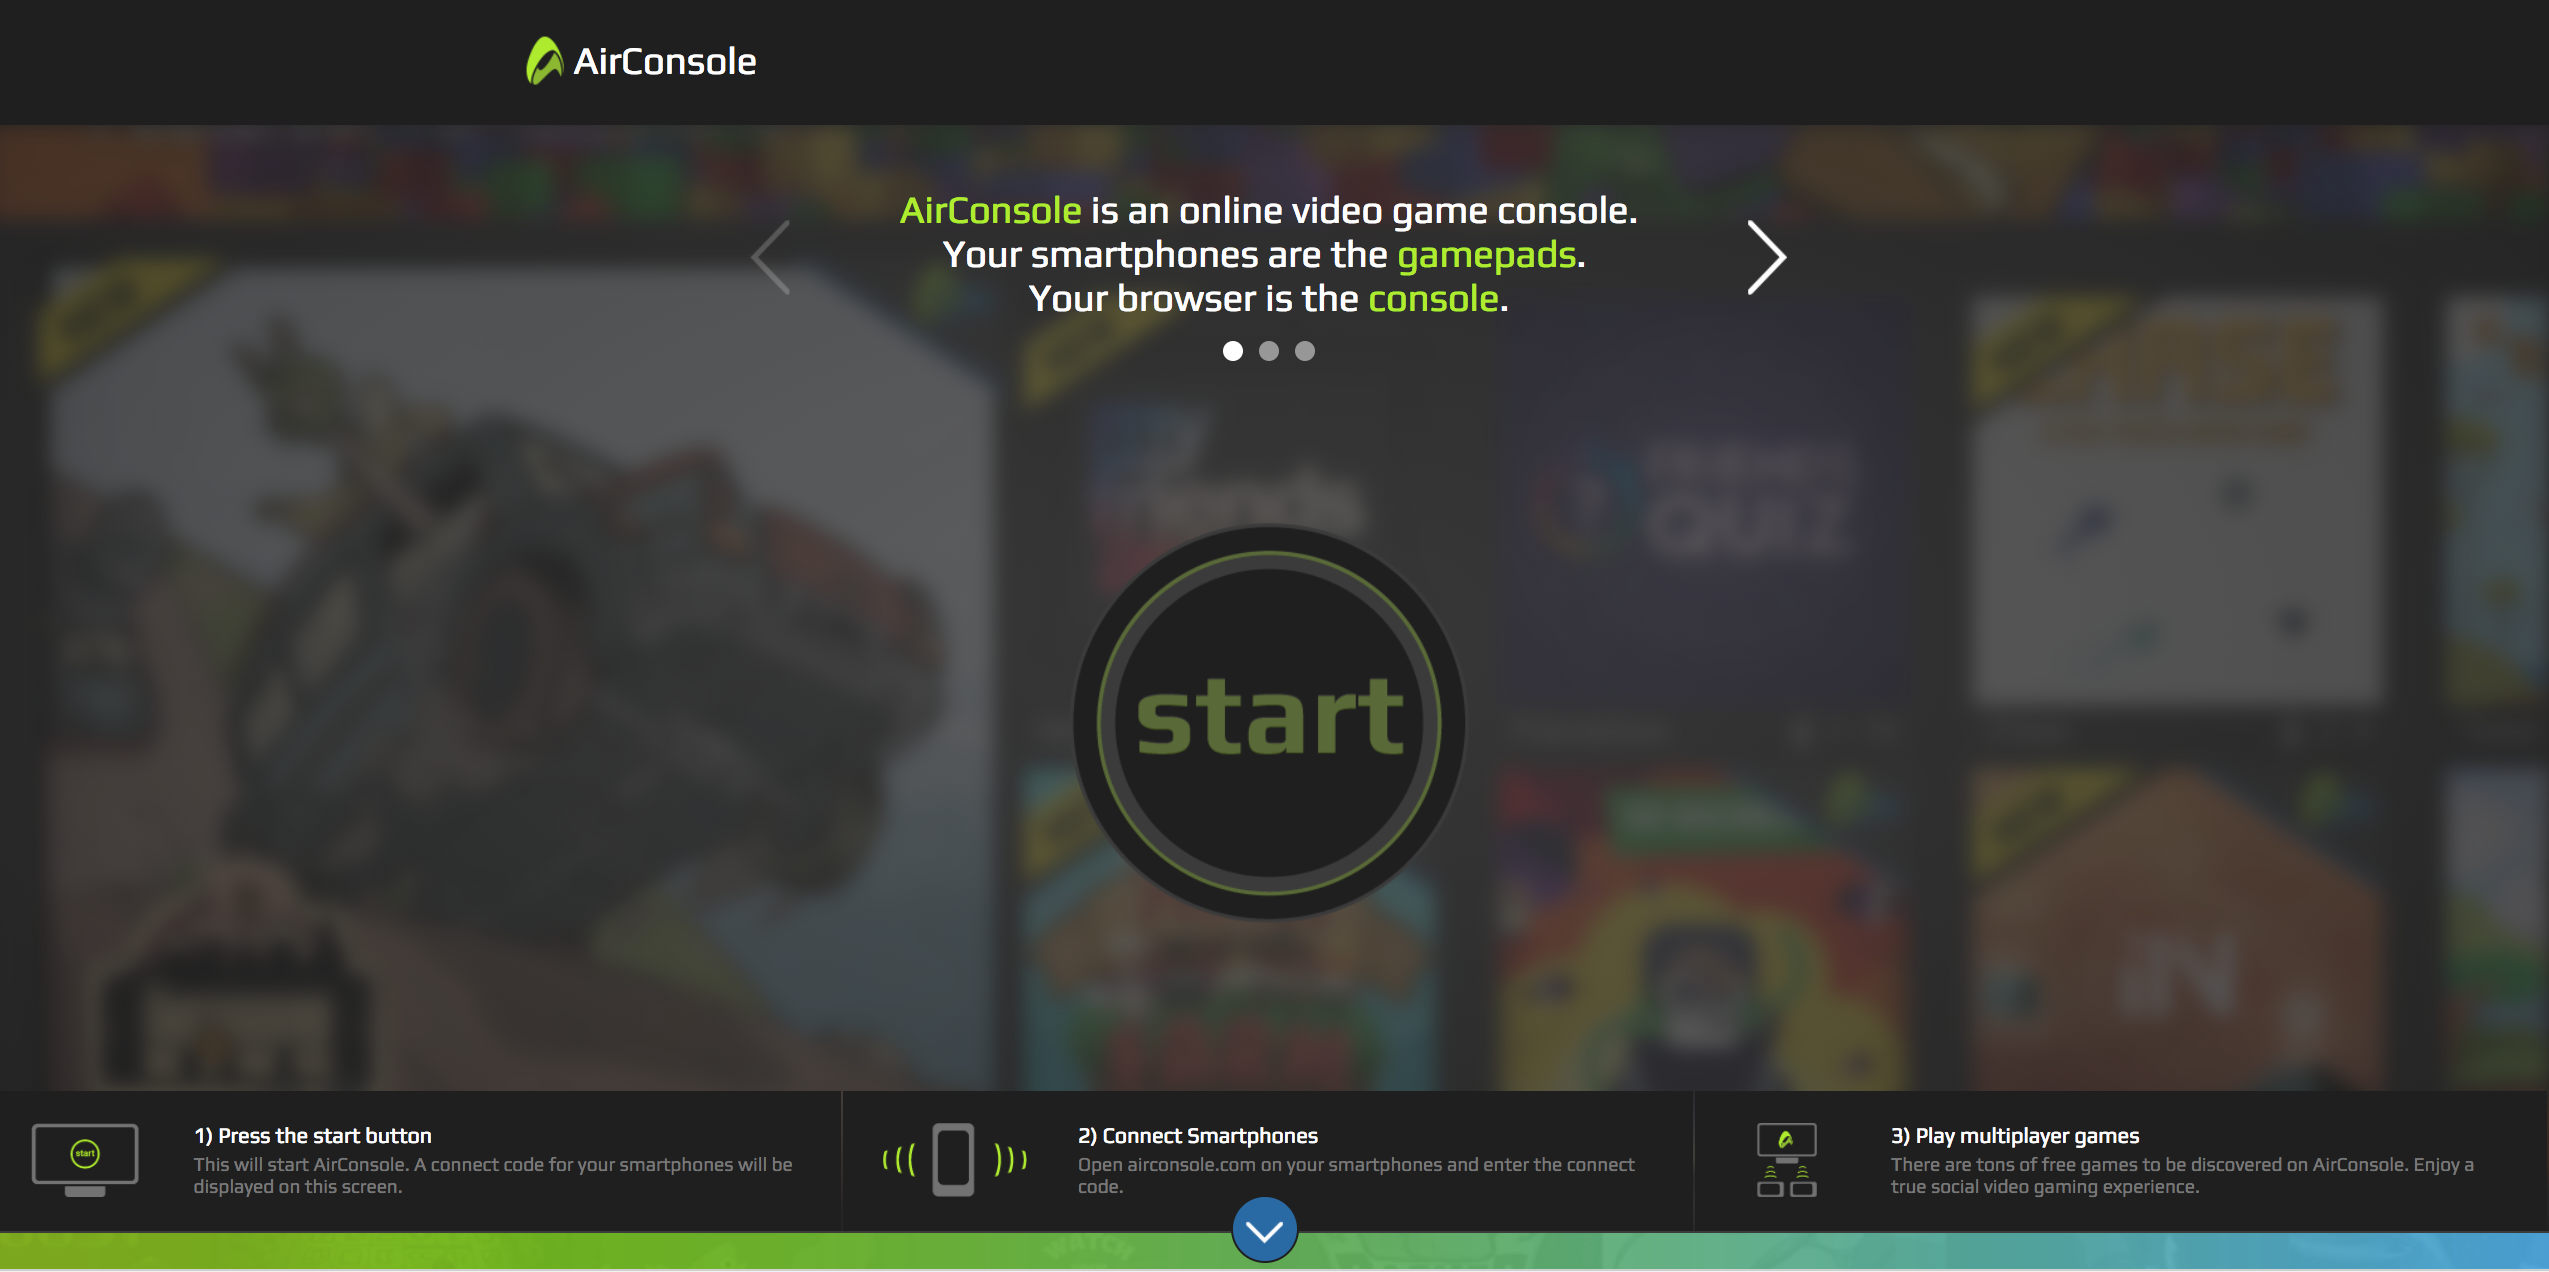
\includegraphics[scale=0.2]{Gambar/con1_home1}
	\caption{Halaman awal web AirConsole pada \textit{PC}.}
	\label{fig:16_con1_home1}
\end{figure}

Setelah tombol \textit{start} ditekan, maka akan muncul halaman berikutnya yang menunjukan kode yang harus dimasukan oleh pemain pada \textit{browser} di \textit{smarthone}. 

\begin{figure}[H]
	\centering
	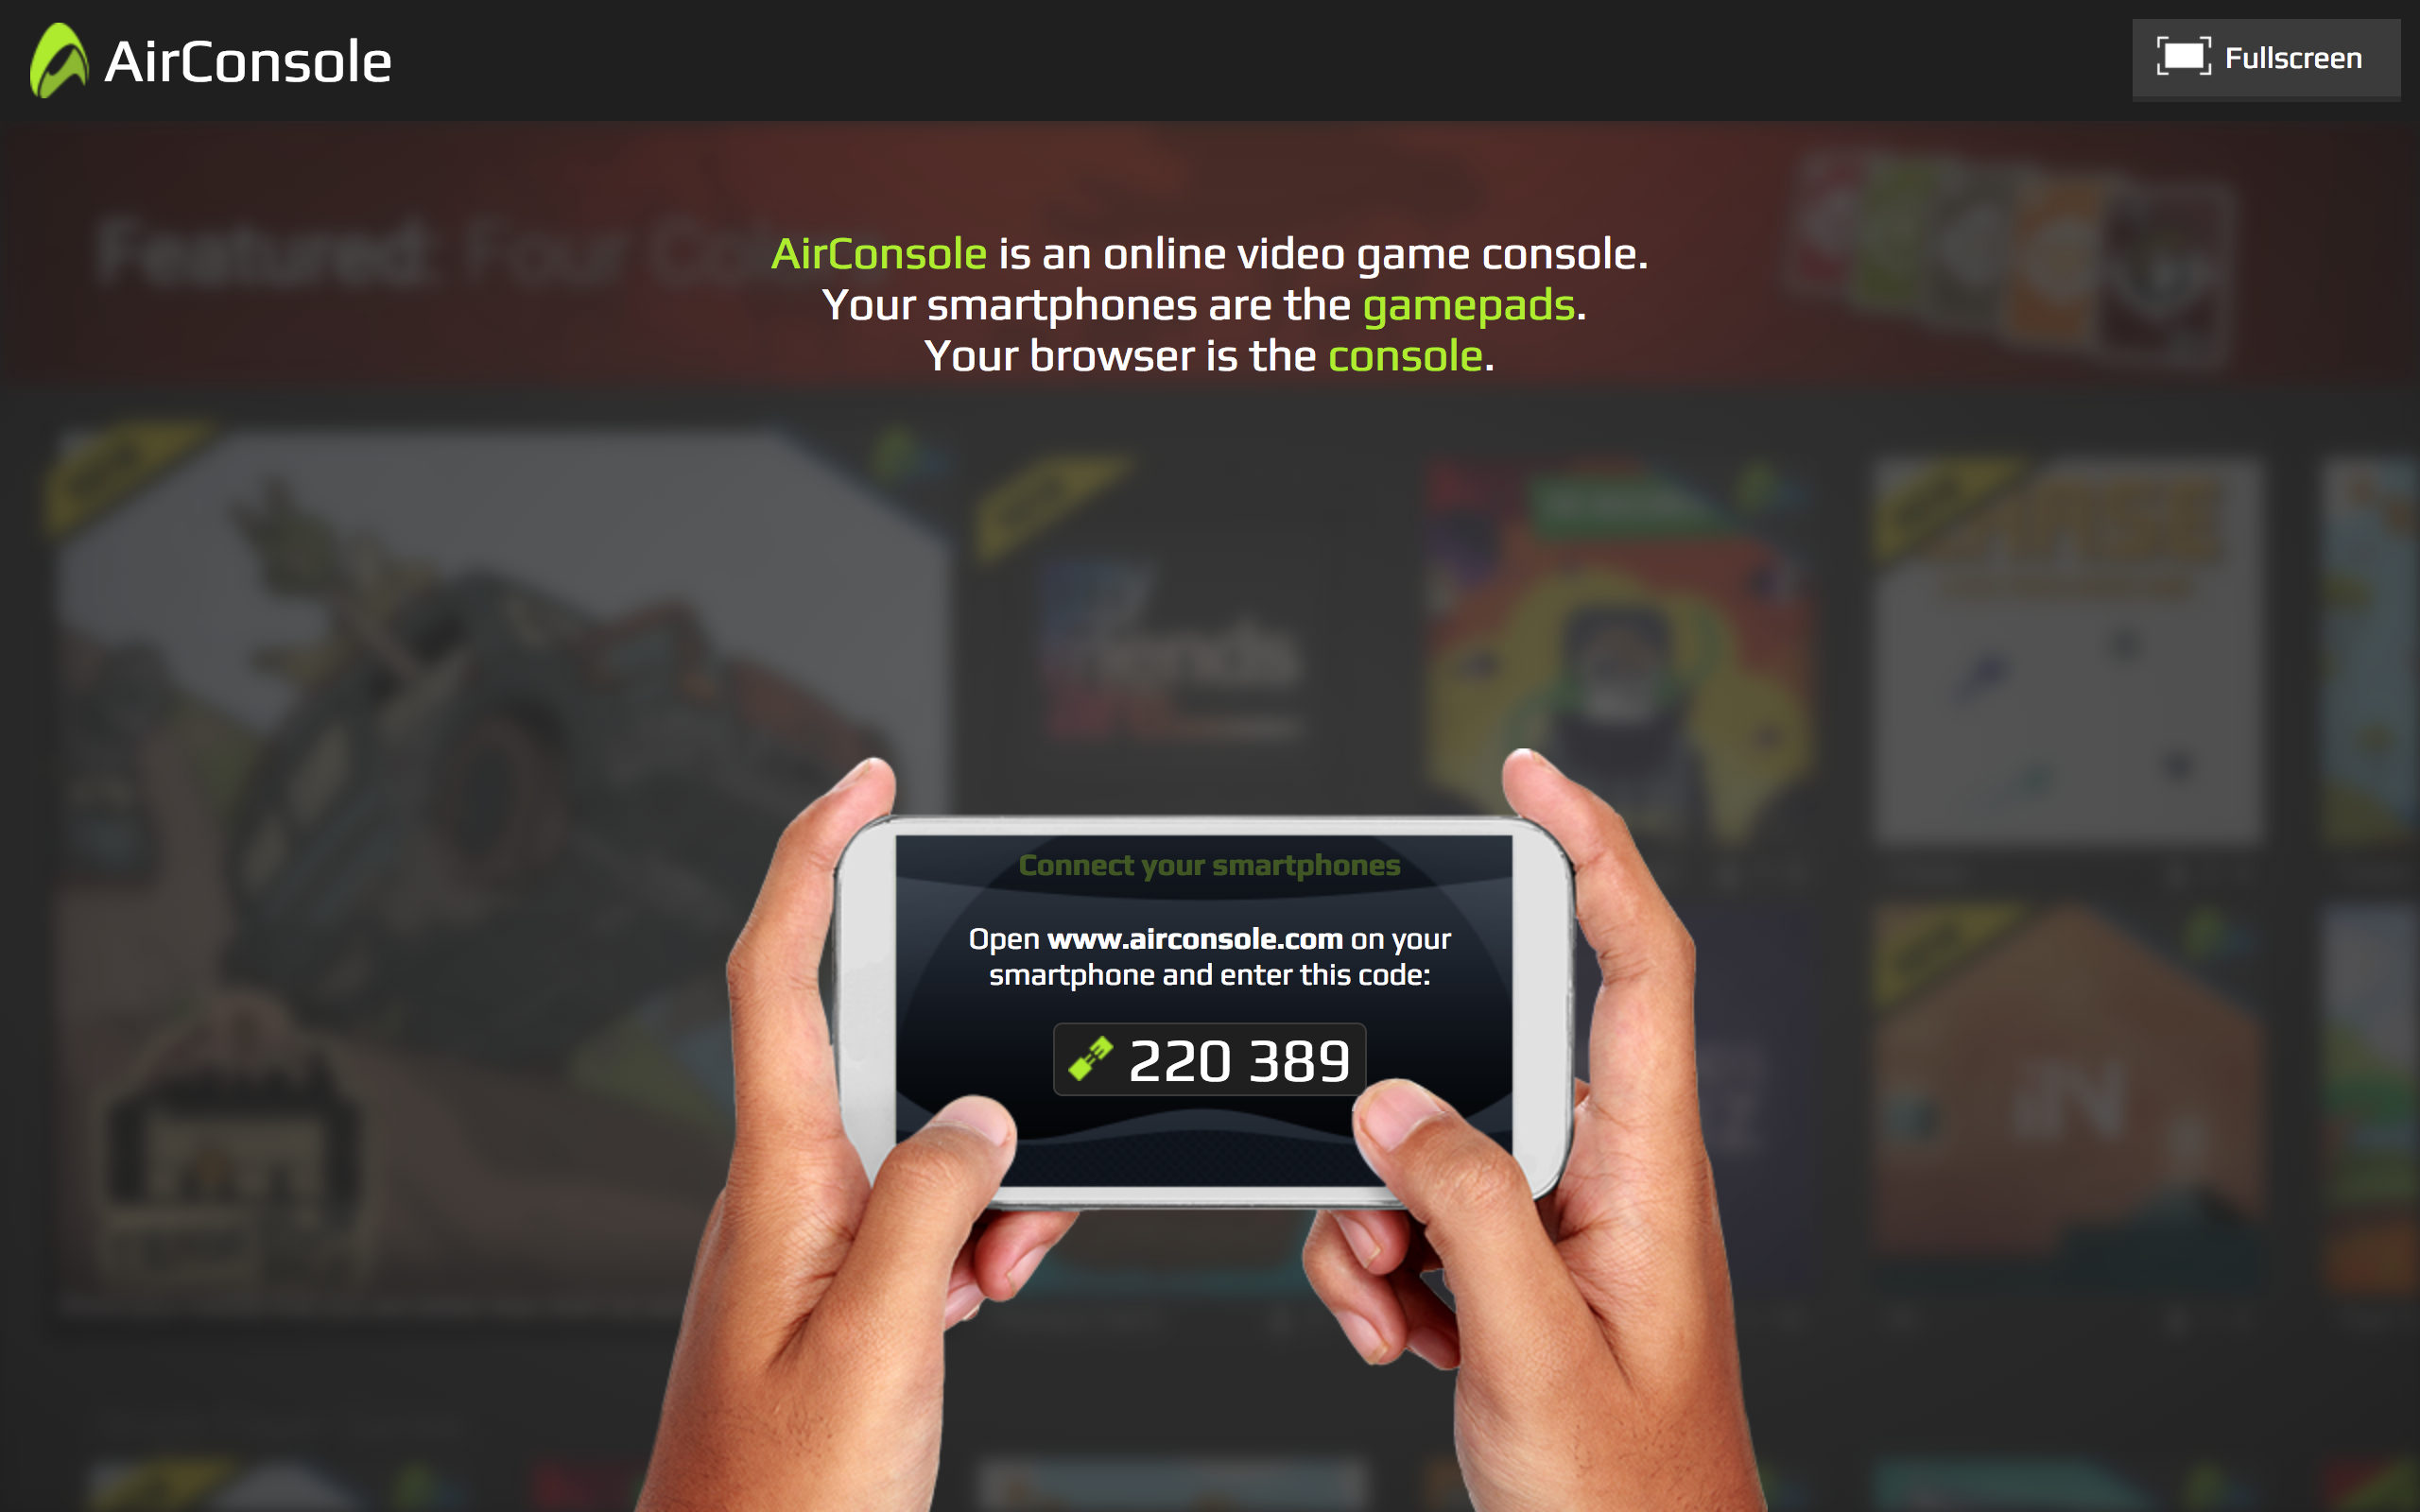
\includegraphics[scale=0.2]{Gambar/con2_code1}
	\caption{Kode yang harus dimasukan oleh pemain pada \textit{smartphone}.}
	\label{fig:17_con2_code1}
\end{figure}

Pemain harus mengakses alamat web yang sama pada \textit{smartphone}. Pada halaman awal, pemain akan diminta untuk memilih apakah akan bermain dengan menggunakan aplikasi, atau bermain dengan menggunakan \textit{browser}. 

\begin{figure}[H]
	\centering
	
\includegraphics[scale=0.2]{Gambar/air1_home}
	\caption{Halaman awal Airconsole pada \textit{smartphone}.}
	\label{fig:18_air1_home}
\end{figure}

%\vspace{-3cm}

Dalam analisis ini, penulis memilih untuk bermain menggunakan \textit{browser}. Setelah itu, pemain diminta untuk menekan tombol \textit{'i got the connect code'} untuk memasukan kode yang sudah didapatkan pada \textit{PC}.

\begin{figure}[H]
	\centering
	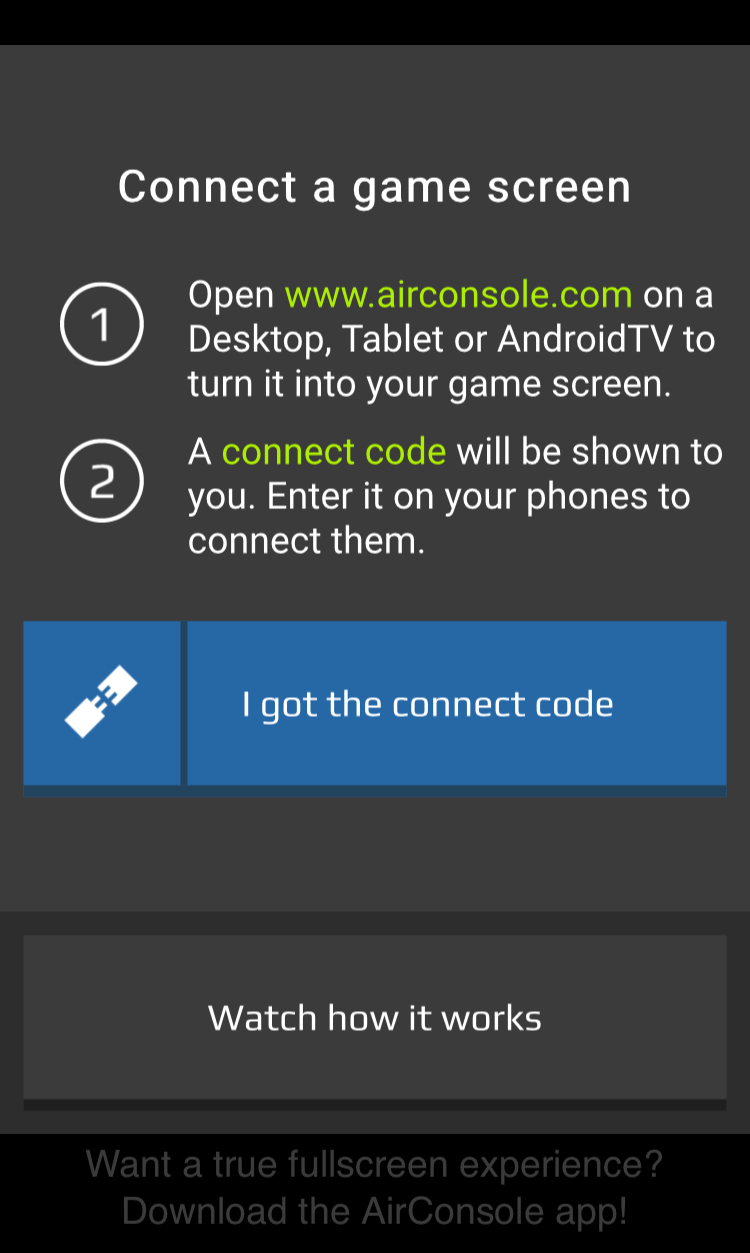
\includegraphics[scale=0.2]{Gambar/air2_code1}
	\caption{Pemain diminta untuk memasukan kode yang sudah didapatkan pada \textit{PC}.}
	\label{fig:19_air2_code1}
\end{figure}


Setelah menekan tombol tersebut, pemain dapat mulai memasukan kode yang sudah didapatkan. Kode ini bertujuan untuk proses verifikasi, sehingga para pemain yang dapat bermain dalam satu sesi yang sama, hanya para pemain yang mengetahui kode tersebut.

\begin{figure}[H]
	
	\centering
	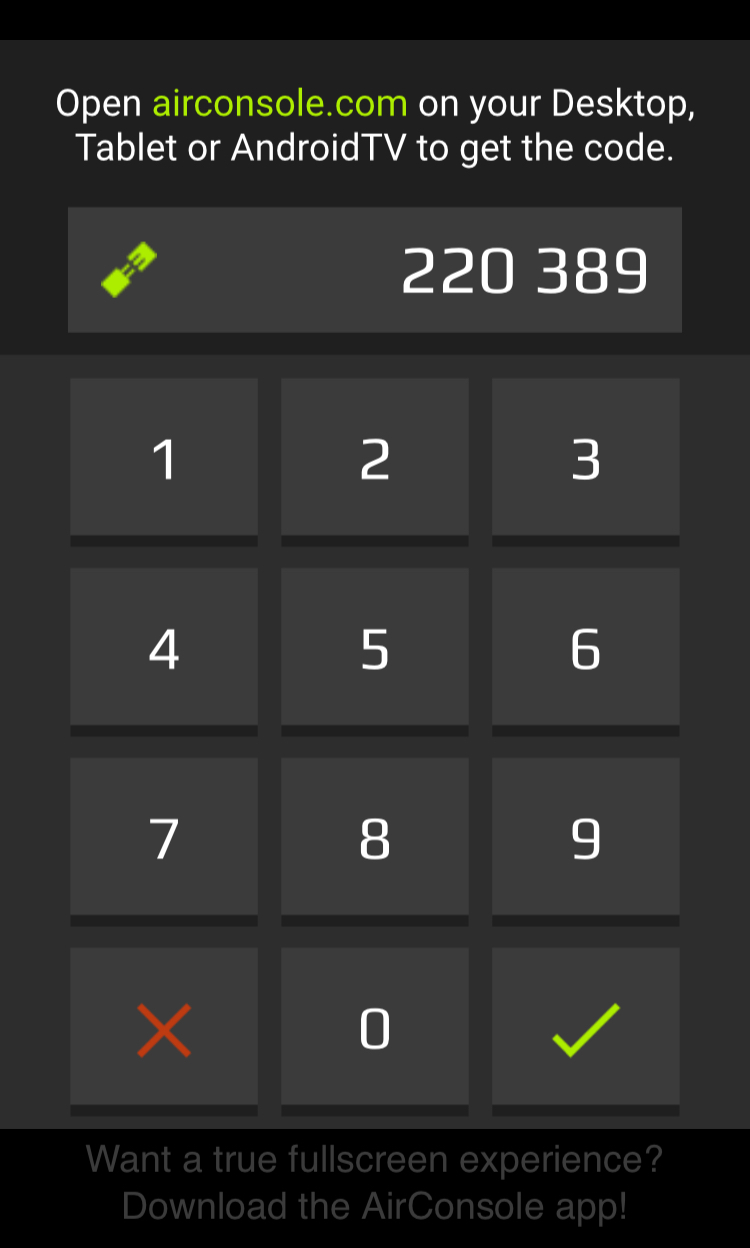
\includegraphics[scale=0.2]{Gambar/air3_code2}
	\caption{Memasukan kode yang sudah didapatkan pada \textit{PC}.}
	\label{fig:20_air3_code2}
	
	
\end{figure}


Setelah pemain memasukan kode, maka halaman web di \textit{PC} dan \textit{smartphone} akan berubah. Pada \textit{PC}, halaman akan menunjukan berbagai jenis permainan yang dapat dipilih. Pada \textit{smartphone}, halaman akan berubah menjadi pengendali permainan, dimana pemain dapat menggerakan halaman yang ada di \textit{PC} dengan menggunakan \textit{smartphone}.

\begin{figure}[H]
	\centering
	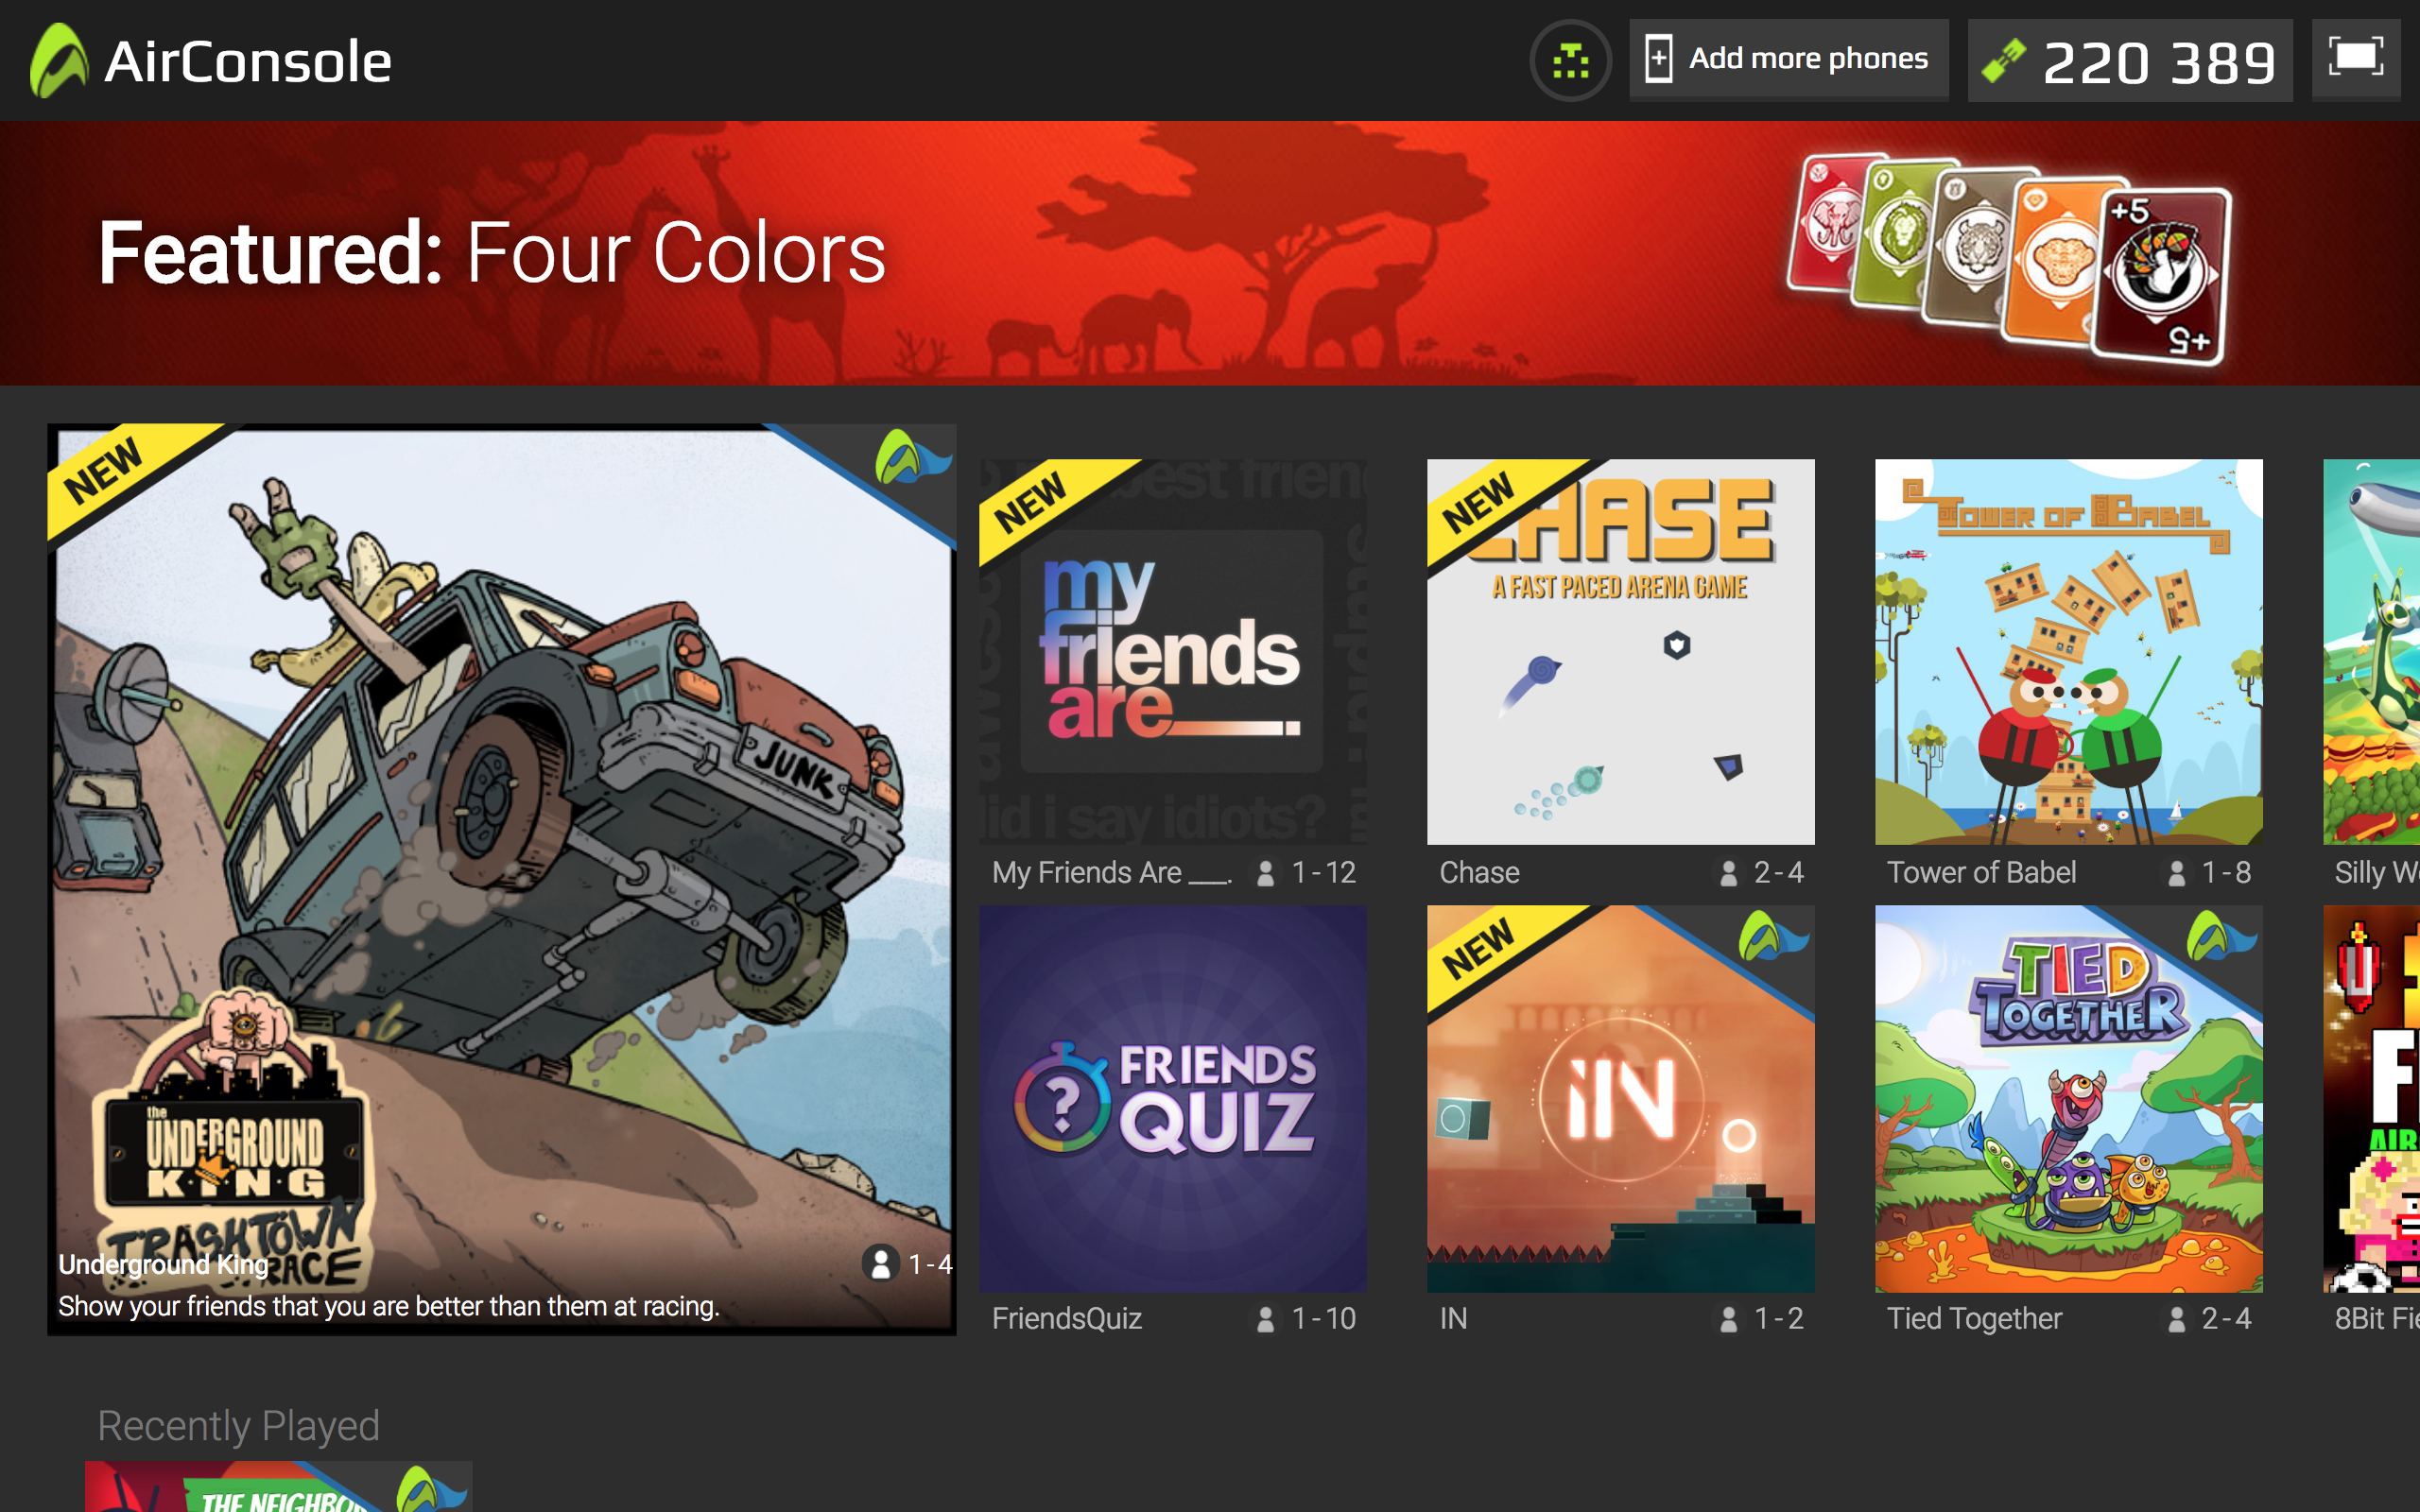
\includegraphics[scale=0.2]{Gambar/con3_play1}
	\caption{Halaman pada \textit{PC} yang menunjukan berbagai permainan yang dapat dipilih.}
	\label{fig:21_con3_play1}
\end{figure}

\begin{figure}[H]
	\centering
	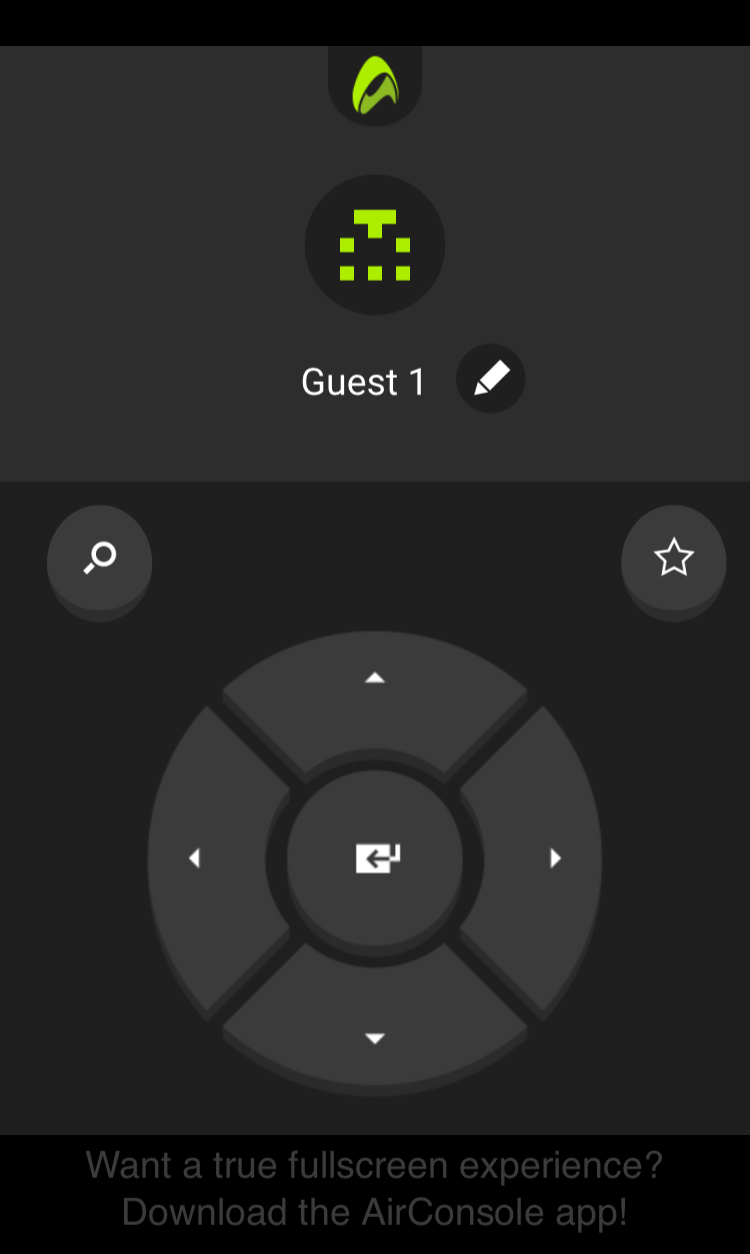
\includegraphics[scale=0.2]{Gambar/air4_play1}
	\caption{Halaman pada \textit{smartphone} yang berfungsi sebagai pengendali.}
	\label{fig:22_air4_play1}
\end{figure}

Dalam analisis ini, penulis memilih untuk memainkan permainan yang bernama The Neighborhood. Permainan ini sejenis permainan Angry Birds. Permainan ini bercerita tentang dua kelompok yang bertetangga, dimana kelompok tersebut bermusuhan dan berusaha untuk saling menghancurkan satu sama lain. Tujuan dari permainan ini yaitu lebih dulu menghancurkan anggota kelompok tetangga. Setelah memilih permainan tersebut, halaman pada \textit{PC} dan \textit{smartphone} akan berubah. Pada \textit{smartphone}, pemain akan diminta untuk merubah mode tampilan \textit{smartphone} menjadi \textit{landscape}.

\begin{figure}[H]
	\centering
	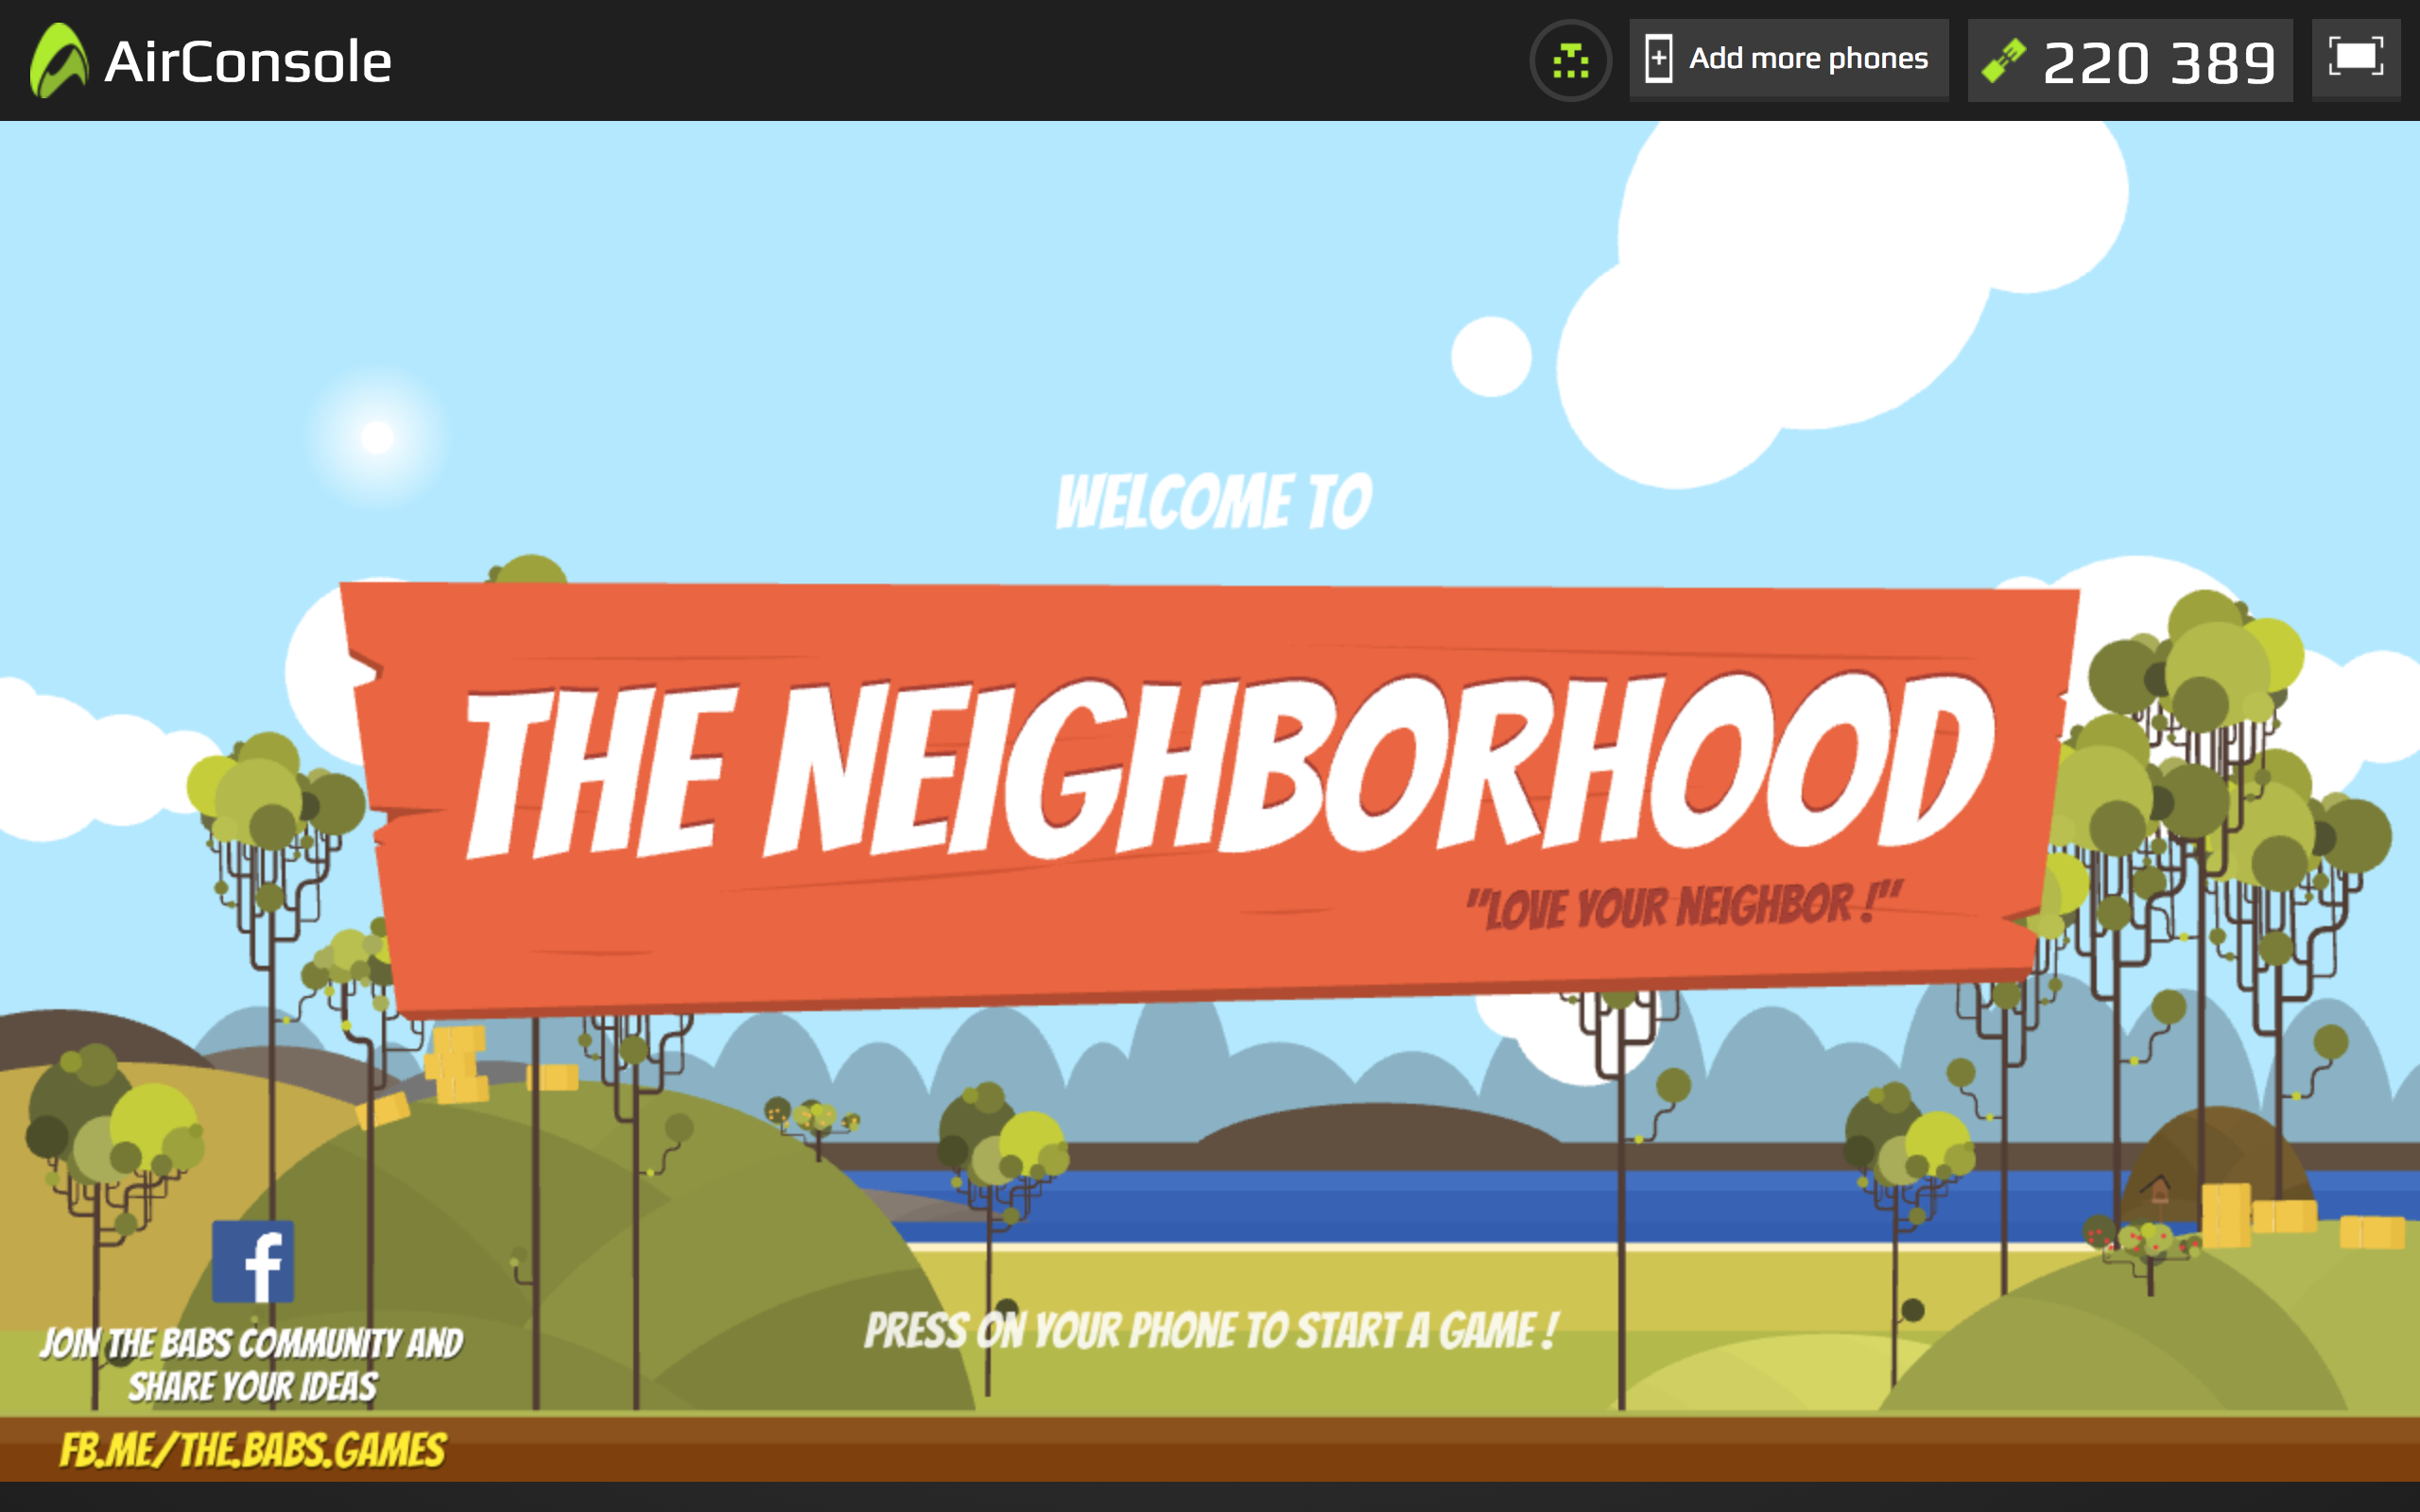
\includegraphics[scale=0.2]{Gambar/con5_play3}
	\caption{Halaman awal permainan The Neighborhood pada \textit{PC}.}
	\label{fig:23_con5_play3}
\end{figure}

\begin{figure}[H]
	\centering
	
\includegraphics[scale=0.2]{Gambar/air6_play3}
	\caption{Halaman awal permainan The Neighborhood pada \textit{smartphone}.}
	\label{fig:24_air6_play3}
\end{figure}

Cara bermain dari permainan tersebut yaitu dengan menggunakan \textit{smartphone}, dimana pemain harus menekan layar \textit{smartphone}, kemudian menariknya sesuai dengan arah yang berlawanan dengan lawan, lalu melepas jari dari layar \textit{smartphone} dengan tujuan untuk melempar suatu benda dari ketapel. Semakin jauh pemain menarik, maka lontaran benda tersebut akan semakin kencang mengenai lawan.

\begin{figure}[H]
	\centering
	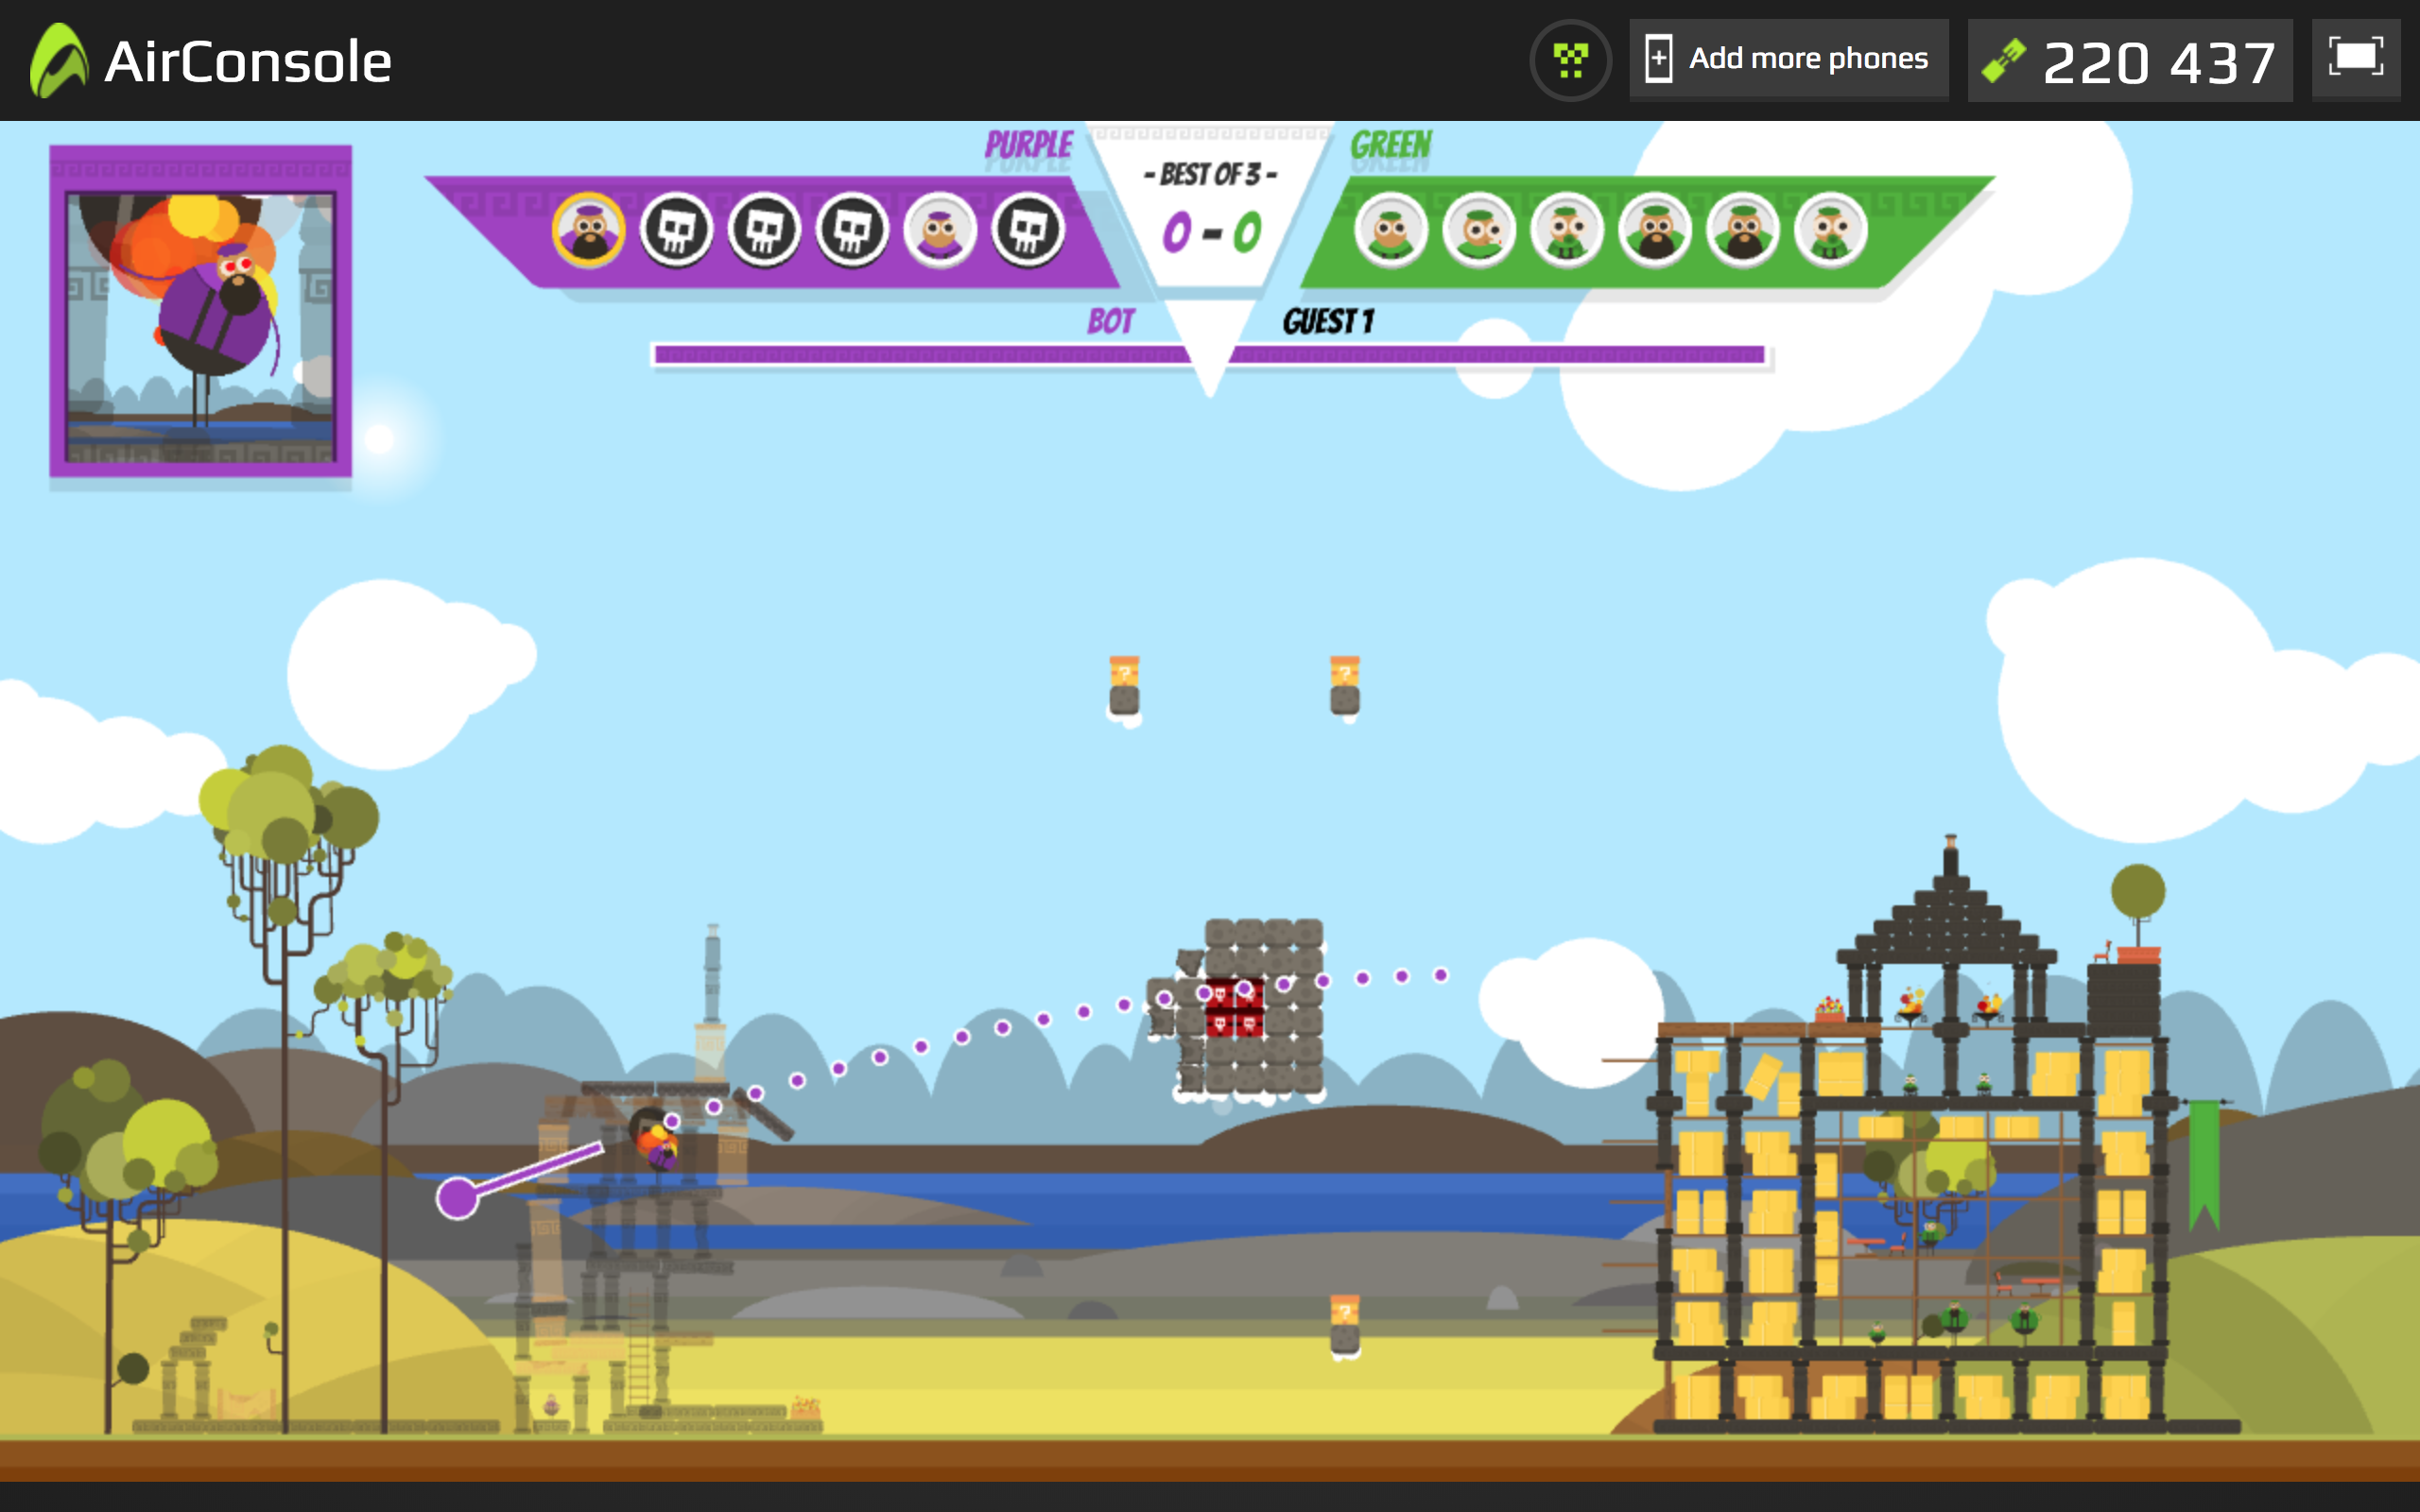
\includegraphics[scale=0.2]{Gambar/con7_play5}
	\caption{Halaman pada \textit{PC} dimana permainan sedang berlangsung.}
	\label{fig:25_con7_play5}
\end{figure}

\begin{figure}[H]
	\centering
	
\includegraphics[scale=0.2]{Gambar/air7_play4}
	\caption{Halaman pada \textit{smartphone} dimana permainan sedang berlangsung.}
	\label{fig:26_air7_play4}
\end{figure}

Pemain dapat memilih untuk keluar dari permainan atau melanjutkan permainanannya kembali setelah menyelesaikan satu level permainan.

\begin{figure}[H]
	\centering
	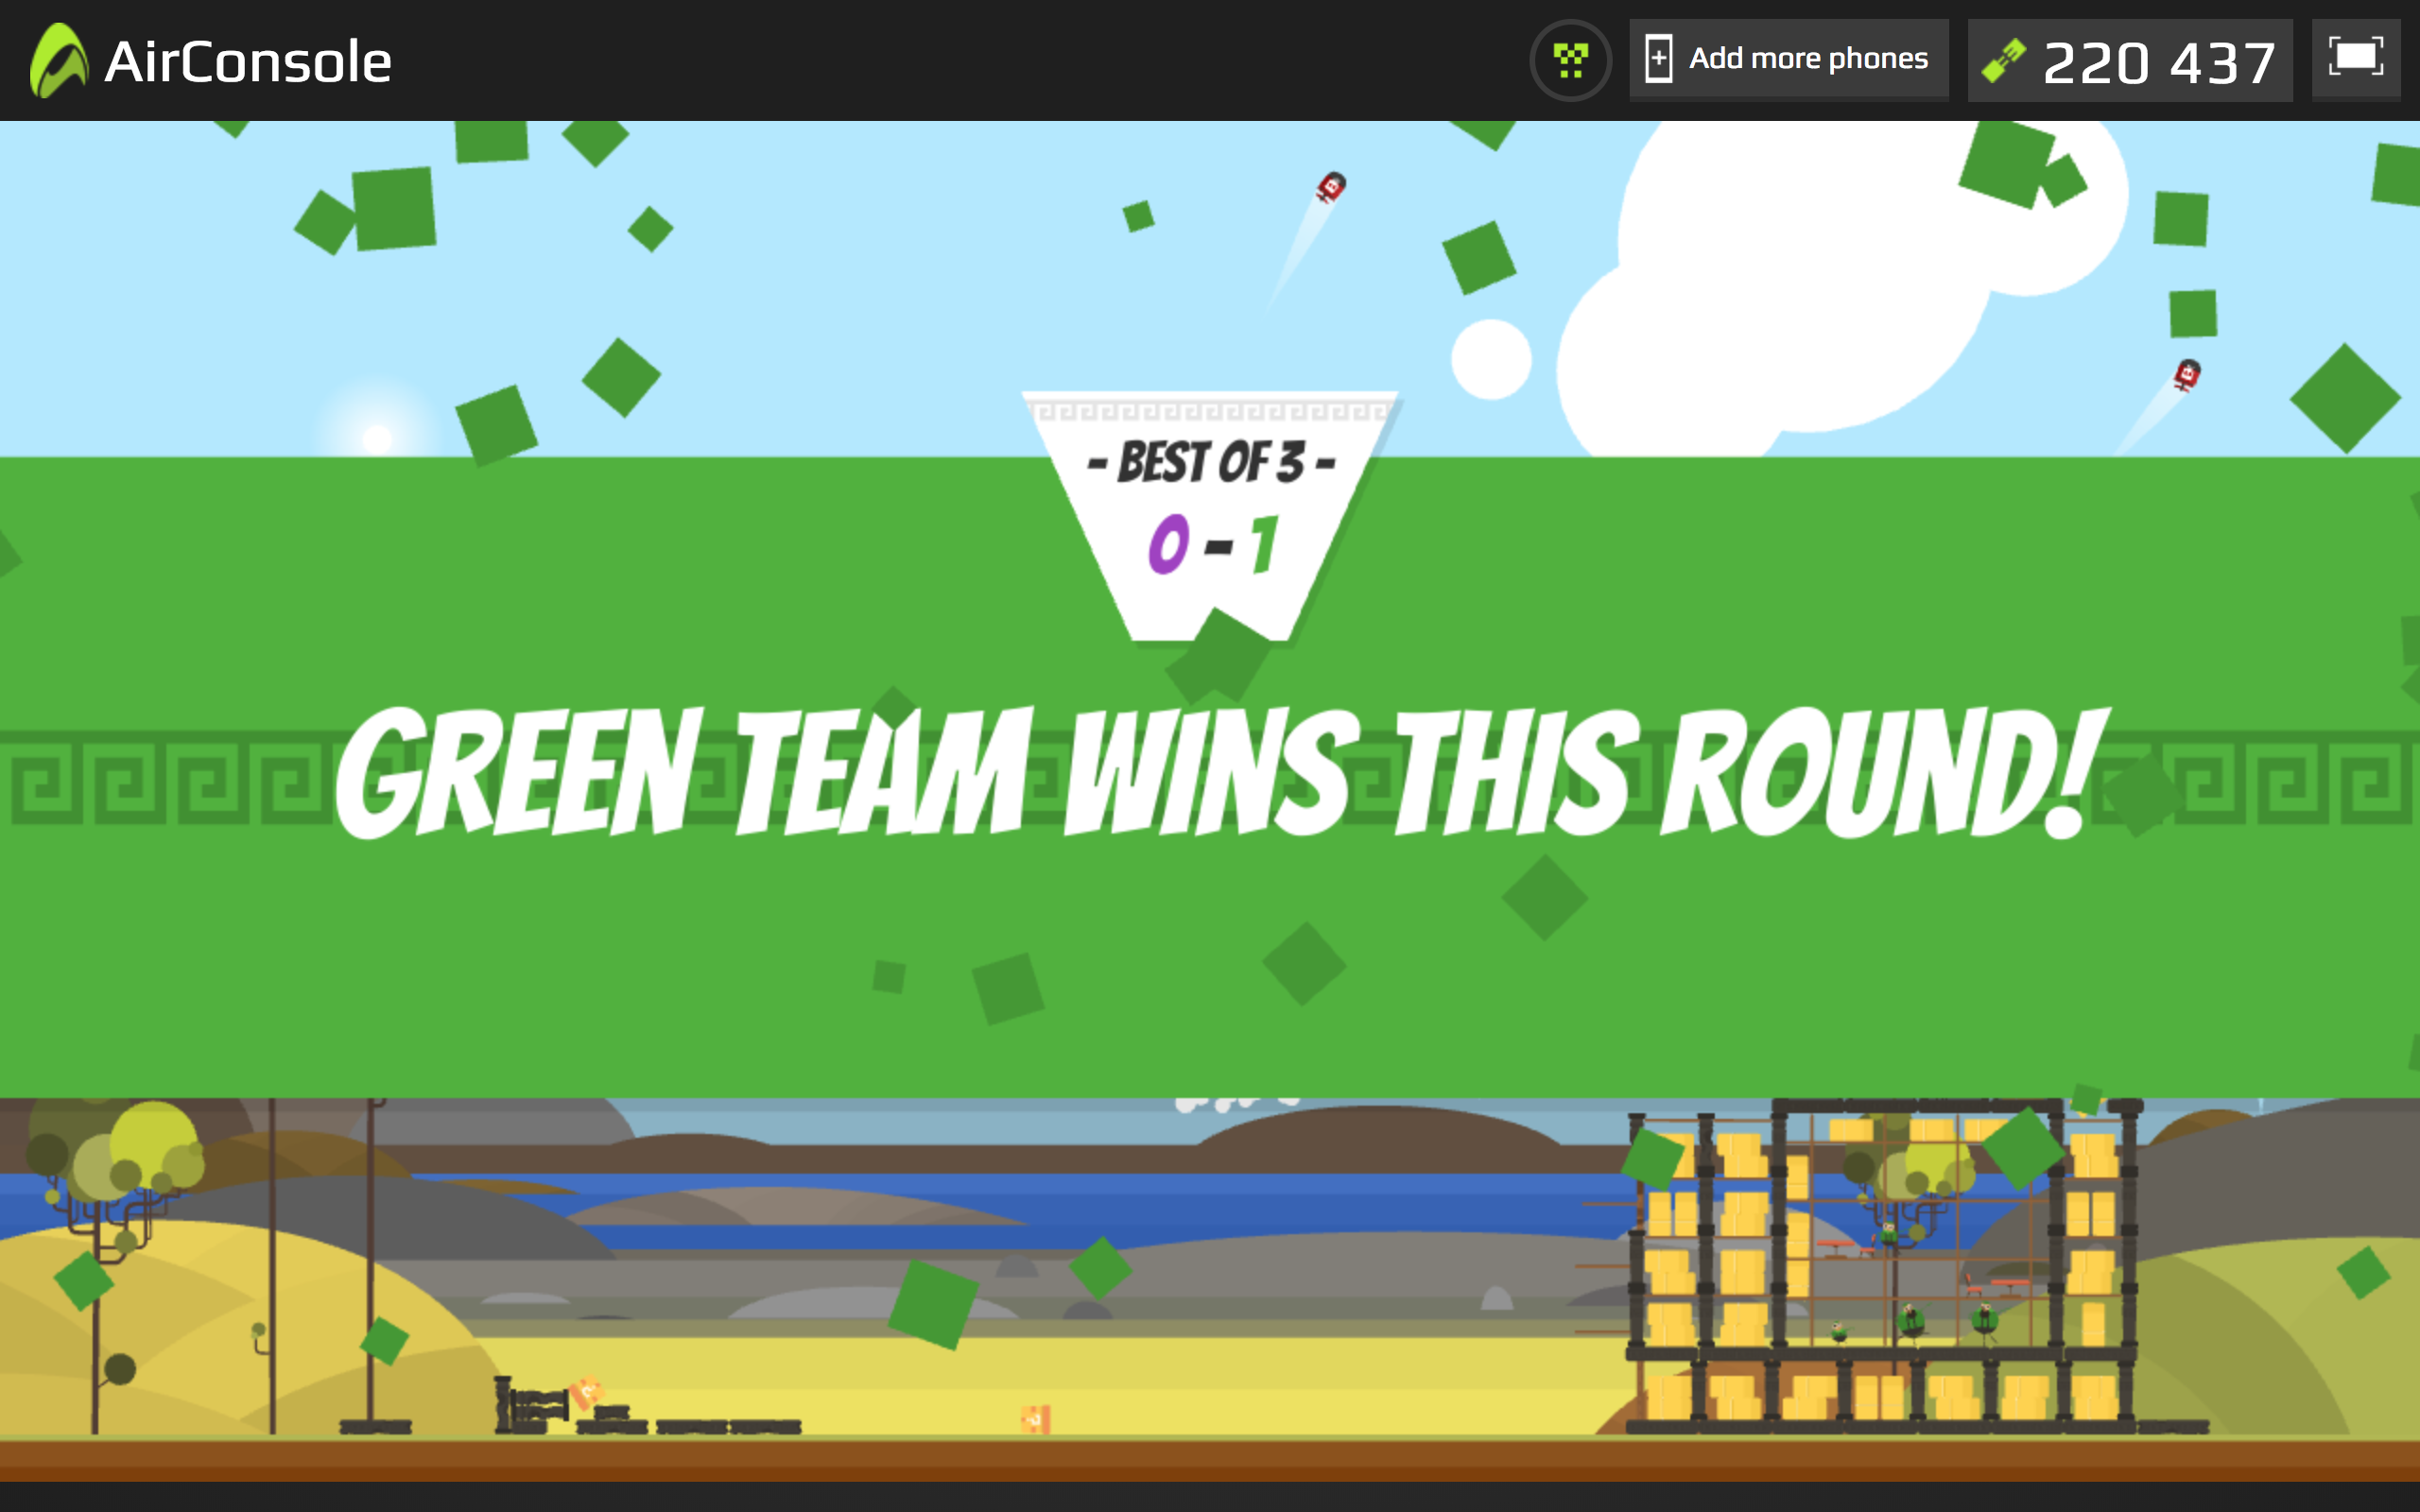
\includegraphics[scale=0.2]{Gambar/con8_play6}
	\caption{Halaman pada \textit{PC} apabila permainan sudah selesai.}
	\label{fig:27_con8_play6}
\end{figure}

\begin{figure}[H]
	\centering
	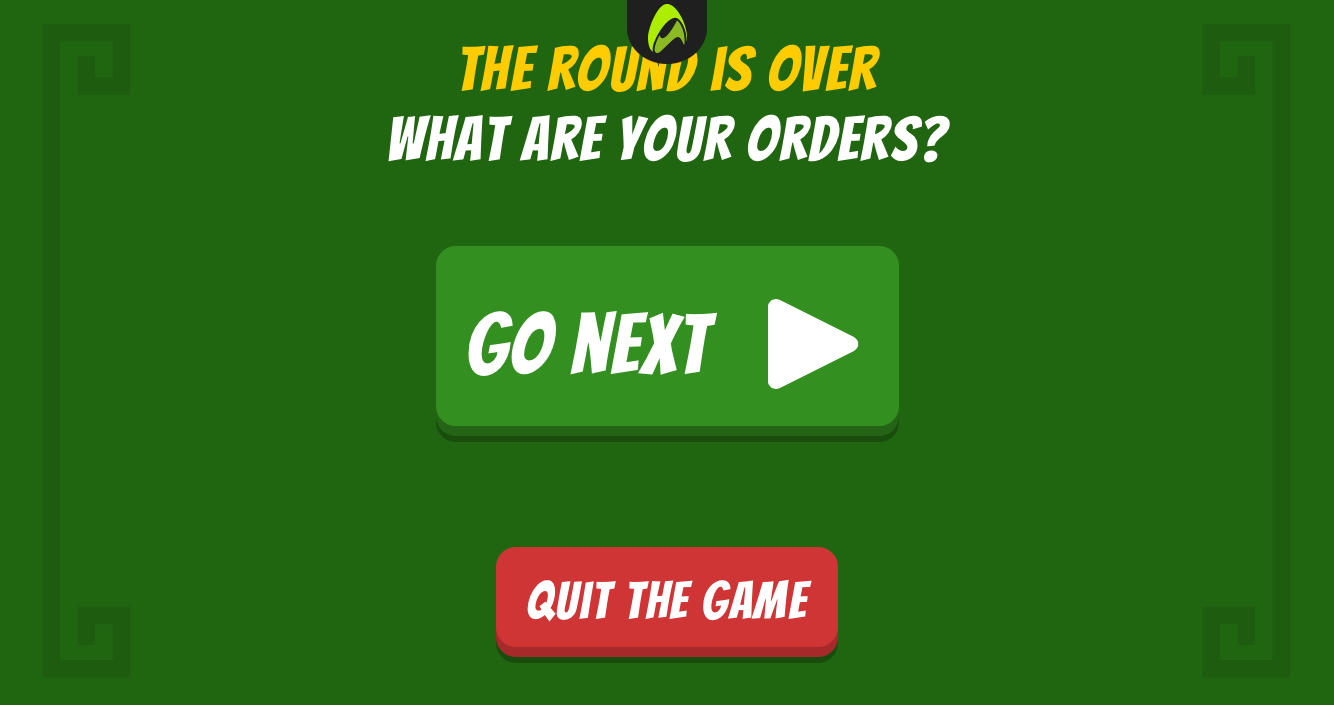
\includegraphics[scale=0.2]{Gambar/air8_finish}
	\caption{Halaman pada \textit{smartphone} apabila permainan sudah selesai.}
	\label{fig:28_air8_finish}
\end{figure}

Dari ketiga percobaan yang sudah dilakukan, ada beberapa hal yang dapat diperbaiki dari permainan berbasis web tersebut. Percobaan pertama menunjukan hasil yang bagus, dimana koneksi antara \textit{smartphone} dan \textit{PC} tidak putus saat permainan berlangsung, dan juga tidak ada keterlambatan antara gerakan pada \textit{smartphone} dan \textit{PC}. Pada percobaan kedua, apabila \textit{browser} pada \textit{PC} ditutup pada saat permainan berlangsung, maka koneksi akan terputus. Tetapi, tampilan pada \textit{smartphone} tidak menunjukan bahwa adanya koneksi yang terputus, sehingga pemain tidak mengetahui apakah permainan masih dapat berlangsung atau tidak. Tampilan hanya akan langsung kembali pada halaman awal permainan. Begitupun dengan percobaan ketiga, apabila \textit{browser} pada \textit{smartphone} ditutup pada saat permainan sedang berlangsung, maka koneksi akan terputus. Tampilan pada \textit{PC} hanya menunjukan tanda kecil bahwa telah terjadi pemutusan koneksi pada \textit{smartphone}, yaitu tanda x pada bagian atas tampilan yang ditunjukan seperti gambar berikut:

\begin{figure}[H]
	\centering
	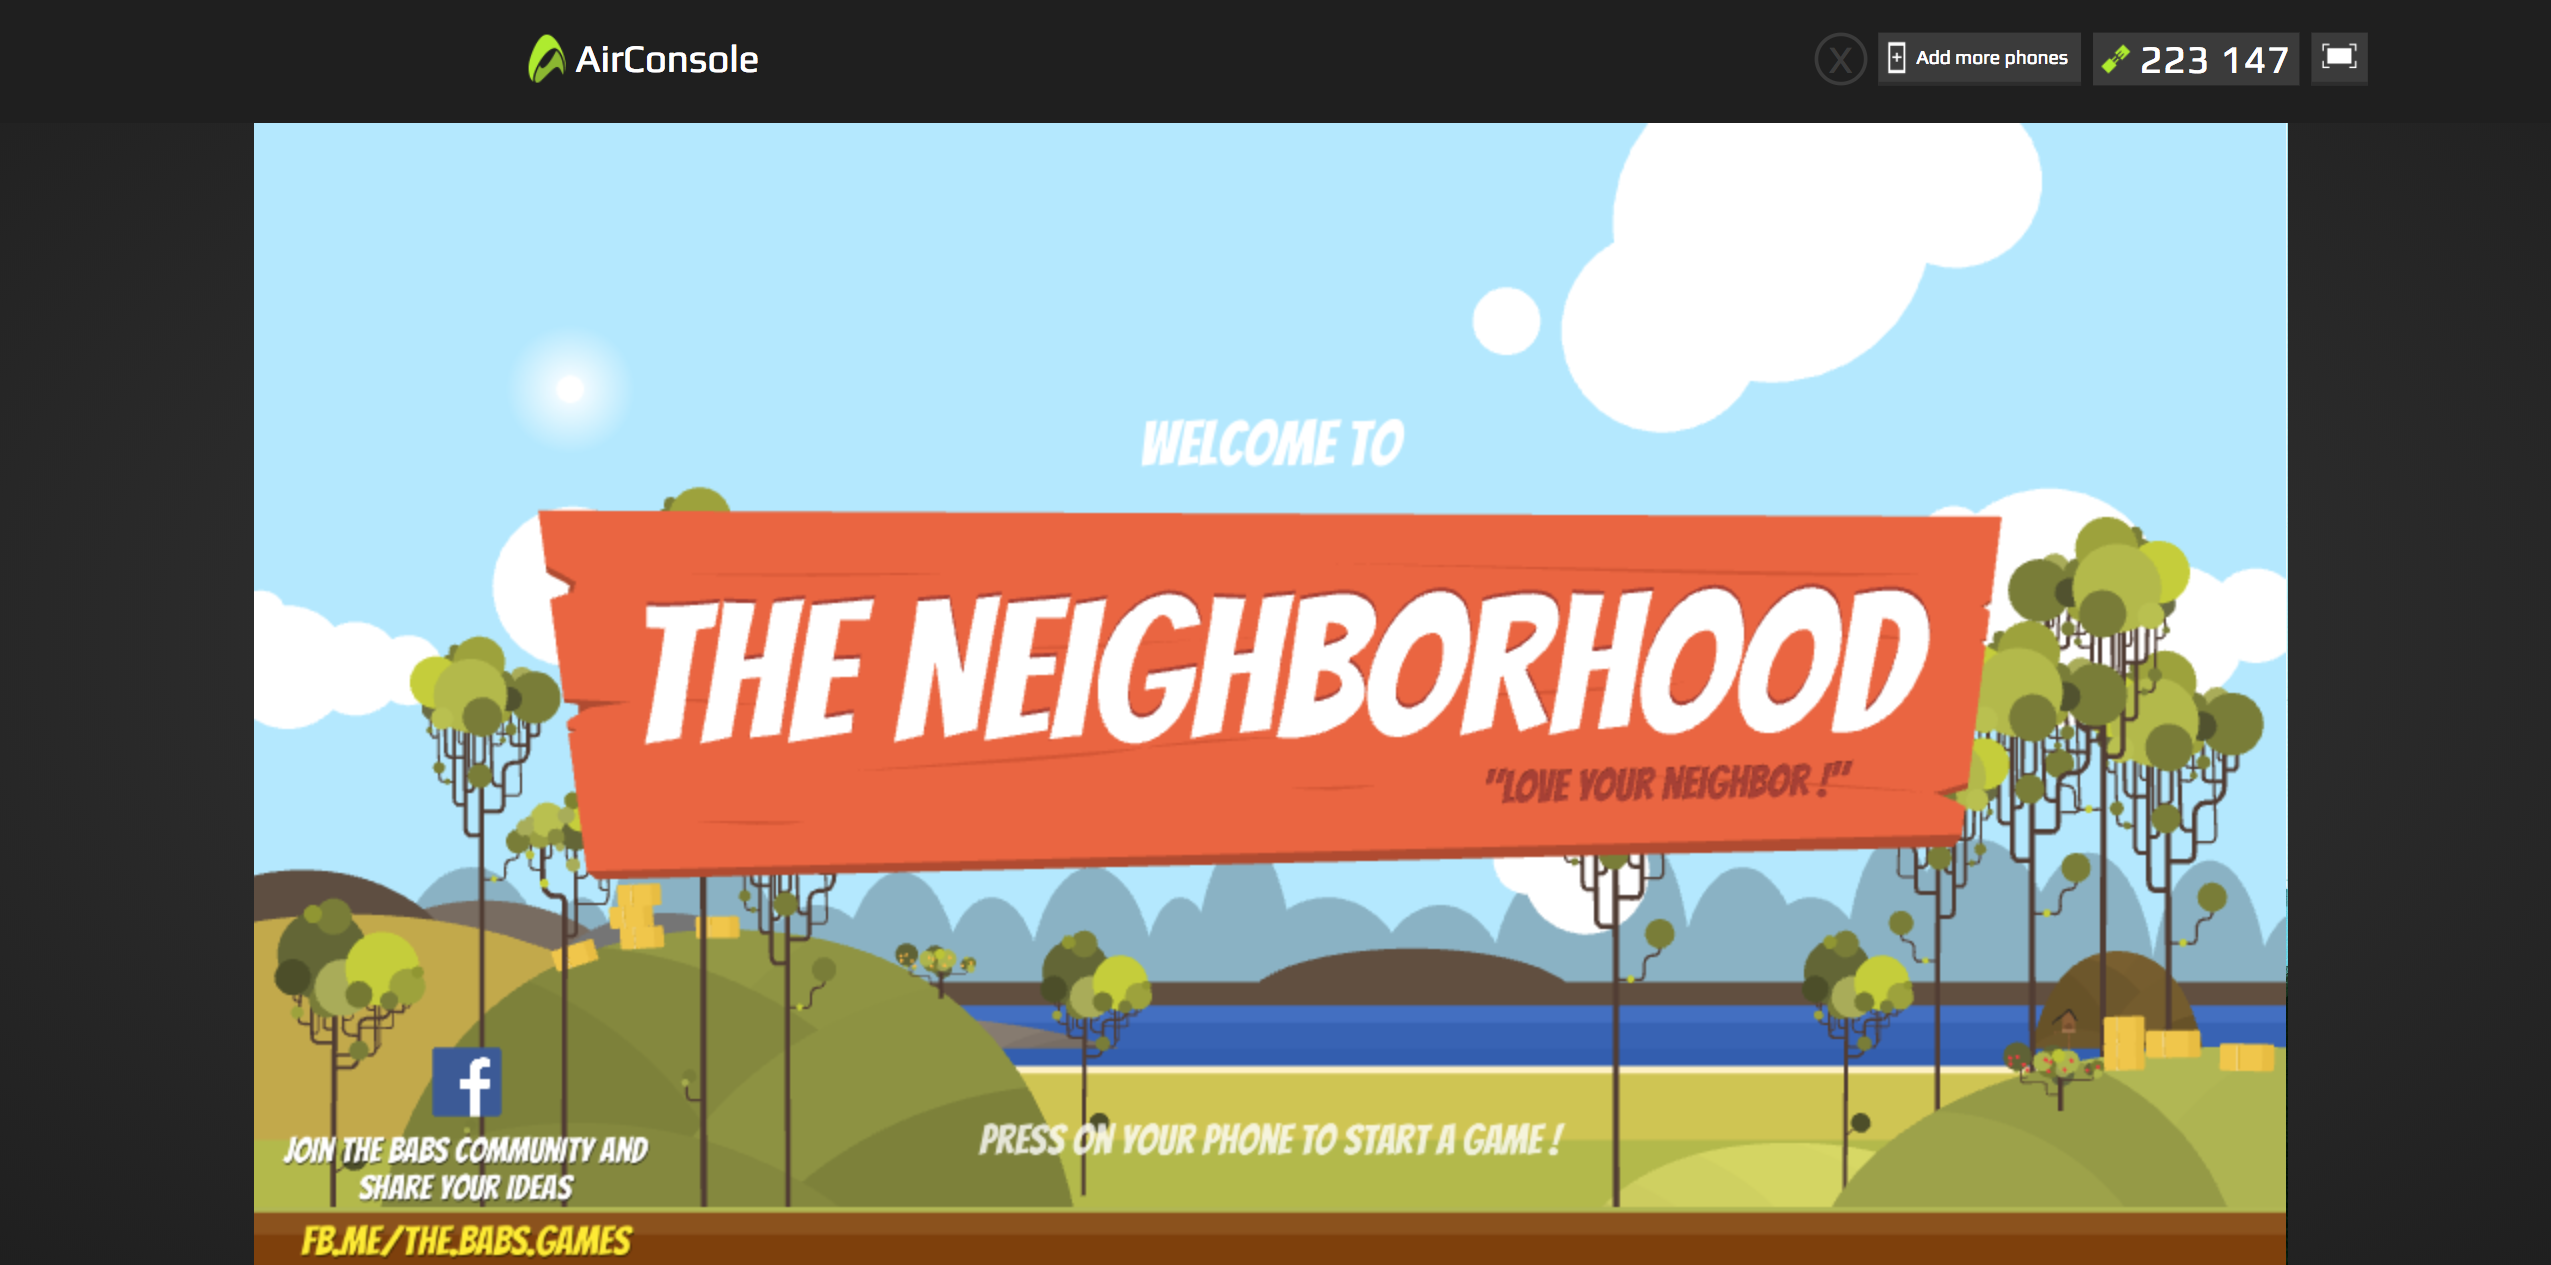
\includegraphics[scale=0.2]{Gambar/con9_play7}
	\caption{Halaman pada \textit{PC} yang menunjukan pemutusan koneksi.}
	\label{fig:29_con9_play7}
\end{figure}

%Perbaikan yang dapat dilakukan adalah dengan memberi \textit{feedback} yang lebih jelas pada pemain, apabila ada kesalahan pada aplikasi yang terjadi seperti pemutusan koneksi. Dengan begitu, pemain akan lebih mengetahui bahwa koneksi dapat saja terputus dan tidak dapat melanjutkan permainannya.

%\section{Analisis Sequence Diagram}
%\label{sequence}
%
%Pada analisis ini dilakukan pengamatan pada jalannya koneksi \textit{socket.io} antara \textit{server} dan \textit{client}. Hal-hal yang dianalisis adalah bagaimana koneksi tersambung di awal permainan, bagaimana data-data yang dibutuhkan dikirim melalui koneksi tersebut, hingga koneksi antara \textit{client} dan \textit{server} terputus. Analisis dilakukan dengan menggunakan \textit{developer tools} yang tersedia pada \textit{web browser} untuk mengamati koneksi \textit{client}, dan \textit{terminal} untuk mengamati koneksi \textit{server}.
%
%%Sediain gambar server dan client saat si host berhasil konek ke socket.io
%
%
%Pada awal permainan, \textit{client} pertama yang melakukan koneksi pada \textit{server} adalah \textit{desktop computer}, yang berperan sebagai \textit{host} dalam permainan.\textit{Host} akan menyediakan suatu kode yang berguna sebagai \textit{room} untuk kedua pemain yang akan bergabung dengan melakukan koneksi ke \textit{server}. \textit{Room} yang disediakan hanya akan menerima tiga \textit{client} saja, yaitu \textit{host}, \textit{player1}, dan \textit{player2}. 
%
%Setelah berhasi melakukan koneksi, maka \textit{client} akan memiliki \textit{socket.id} yang berfungsi sebagai tanda pengenal unik, dan kode \textit{room} dimana proses pengiriman dan penerimaan data hanya dapat dilakukan didalam \textit{room} tersebut. 
%
%Setelah \textit{client} pertama berhasil tersambung, selanjutnya para pemain yang akan bergabung akan melakukan koneksi pada \textit{server}. Pemain akan menggunakan \textit{smartphone} yang akan berfungsi sebagai \textit{controller} permainan. Untuk melakukan koneksi, pemain harus memasukan kode \textit{room} yang telah disediakan \textit{host} agar dapat bergabung. Pada proses ini, akan dilakukan pengecekan oleh \textit{server}, apakah kode \textit{room} yang telah dikirim oleh \textit{client} tersedia atau tidak. Apabila \textit{room} tersedia, maka pemain akan berhasil bergabung, dan apabila tidak tersedia, maka pemain tidak dapat bergabung.
%
%Pengecekan tambahan yang dilakukan pada proses ini adalah jumlah \textit{client} yang sudah ada didalam \textit{room}. Apabila jumlahnya masih kurang dari tiga, maka \textit{room} masih membuka koneksi bagi yang akan bergabung. Apabila \textit{room} sudah diisi oleh tiga \textit{client}, maka \textit{room} tidak akan menerima \textit{client} yang akan bergabung lagi.
%
%%sediain gambar client dan sever saat si pemain request connection 
%
%Pada tahap ini, halaman pada \textit{client} dan \textit{server} akan menuju ke halaman pemilihan karakter. Pada jalannya permainan, \textit{socket.id} yang dimiliki oleh masing-masing \textit{client} akan berperan sangat penting untuk proses pengiriman data. Pada koneksi \textit{socket.io}, apabila suatu \textit{client} berpindah halaman dari satu \textit{file} \textit{html} menuju \textit{file} \textit{html} lainnya, koneksi tersebut akan terputus dan akan melakukan koneksi ulang kembali. Dengan begitu, \textit{socket.id} yang dimiliki oleh \textit{client} pun akan berganti karena proses perpindahan \textit{file} \textit{html} dan koneksi ulang. 
%
%Agar koneksi yang dimiliki \textit{client} tidak terputus dan \textit{socket.id} yang dimiliki tidak berganti, maka untuk proses perpindahan halaman harus dibutuhkan satu \textit{file} \textit{html} saja. Hal tersebut dapat dilakukan dengan cara menggunakan \textit{syntax} yang disediakan oleh \textit{html}, yaitu \textit{template}. 
%
%%sediain gambar screenshot syntax template html untuk macem2 halaman
%
%Dengan menggunakan \textit{template} pada satu \textit{file} \textit{html}, maka proses perpidahan halaman hanya akan terjadi didalam satu \textit{file} saja. Halaman yang akan ditunjukan kepada \textit{client} akan dilakukan dengan cara berpindah dari satu \textit{template} ke \textit{template} yang lainnya. Dengan begitu, koneksi \textit{socket.io} tidak akan terputus, dan \textit{socket.id} milik \textit{client} tidak akan berganti.
%
%Setelah masuk ke halaman pemilihan karakter, pemain dapat memilih karakter yang akan dimainkan. Pada \textit{smartphone}, akan ditampilkan daftar karakter yang dapat dipilih, dan pada \textit{desktop}, akan ditampilkan karakter mana yang telah dipilih oleh para pemain untuk dimainkan.
%
%%sediain gambar smartphone yang isinya daftar pemain, sama desktop yang nunjukin karakter mana yang dipilih.
%
%Agar karakter yang dipilih pada \textit{smartphone} sesuai dengan yang ditunjukan oleh \textit{desktop}, maka dibutuhkan proses pengiriman data didalam koneksi \textit{socket.io}. Saat pemain memilih karakter, pemain akan mengirimkan suatu \textit{event} kepada \textit{server} dengan parameter yang berisi \textit{socket.id} dan \textit{value} yang menandakan karakter mana yang dipilih. Setelah \textit{event} tersebut sampai pada \textit{server}, akan dilanjutkan kembali kepada \textit{client} yang berperan sebagai \textit{host}. Pada tahap ini, \textit{host} akan menerima \textit{event} tersebut dan memprosesnya. Parameter \textit{value} yang dikirimkan oleh pemain dibutuhkan oleh \textit{host} untuk menampilkan karakter yang dipilih, sedangkan \textit{socket.id} berfungsi untuk mengetahui pemain mana yang memilih karakter tertentu sehingga dapat menampilkannya dengan tepat.
%
%%sediain gambar screenshot code event charSelecting, terus tampilin juga dev tools sama terminal
%
%Setelah karakter ditampilkan pada \textit{desktop}, maka pemain dapat menekan tombol \textit{choose} yang berarti pemain sudah memutuskan untuk memakai karakter tersebut di permainan. Pada proses ini, akan dilakukan pengecekan pada \textit{server}, apakah kedua pemain sudah menetapkan karakter yang akan dimainkan. Apabila belum ada atau hanya satu pemain yang sudah menetapkan karakter, maka permainan belum bisa dimulai. Permainan akan dimulai apabila kedua pemain telah menetapkan karakter, yang kemudian halaman akan berpindah pada halaman permainan.
%
%%sediain gambar pengecekan udah ada pemain yang milih atau belum.
%
%Kedua pemain yang telah menetapkan karakter akan ditampilkan halaman permainan, begitu juga dengan \textit{host}. Pada halaman \textit{desktop}, pertama-tama akan ditampilkan \textit{countdown} selama tiga detik sebelum para pemain dapat menggunakan \textit{smartphone}nya sebagai \textit{controller}. Apabila \textit{countdown} sudah habis, maka permainan dapat dimulai.
%
%Pemain akan menekan tombol yang ditampilkan di \textit{smartphone} secara terus menerus. Pada tahap ini, apabila tombol ditekan, pemain akan mengirimkan suatu \textit{event} pada \textit{server} dengan parameter berisi \textit{socket.id}. Setelah \textit{event} tersebut sampai ke \textit{server}, maka akan dilanjutkan kembali menuju \textit{client} yang berperan sebagai \textit{host}. \textit{Host} akan memproses \textit{event} tersebut, dan menyesuaikan pemain mana yang memiliki \textit{id} sesuai dengan yang diterima. Karakter akan mulai bergerak sesuai dengan \textit{id} para pemain. Agar karakter yang dimainkan dapat mencapai garis akhir, maka pemain harus menekan tombol pada \textit{smartphone} terus menerus.
%
%%sediain gambar screenshot si player yang neken tombol, terus tampilin terminal yang nunjukin canvas api animation.
%
%Apabila sudah ada pemain yang menyentuh garis akhir, maka permainan pun akan berakhir dan halaman akan berubah menuju ke halaman pemenang. Pada saat permainan berakhir, akan dikirimkan suatu \textit{event} ke \textit{server} yang berisi parameter \textit{socket.id} dan \textit{value} untuk menampilkan pemain mana yang menang dan karakter mana yang dimilikinya. \textit{Event} tersebut kemudian dilanjutkan kembali ke \textit{host} lalu pemenang pun dapat ditampilkan. Pada tahap ini, pemain dapat memilih untuk keluar dari permainan dan kembali ke halaman utama.
%
%%tampilin gambar winning page sama console dan si terminalnya juga



\section{Analisis Alur Permainan Finger For Life}
\label{sec:alur}

Web yang akan dikembangkan merupakan aplikasi permainan berbasis web yang bernama Finger For Life. Jenis permainan ini adalah kompetisi balap lari yang dilakukan oleh dua pemain. Tujuan dari permainan ini adalah mencapai garis akhir lintasan lari lebih dulu untuk menjadi pemenang. Untuk dapat memainkan permainan ini, para pemain harus menyiapkan beberapa hal seperti berikut:

\begin{itemize}
	\item \textbf{Satu Komputer \textit{PC}}.
	\item \textbf{Dua \textit{smartphone}}.
	\item \textbf{Jaringan Internet}.
\end{itemize}

Para pemain harus menyediakan satu perangkat komputer \textit{PC}, dimana \textit{PC} tersebut akan berfungsi sebagai \textit{console}, dan dua \textit{smartphone} yang akan berfungsi sebagai \textit{controller}. \textit{PC} akan memiliki peran sebagai \textit{host} yang menciptakan suatu \textit{room}, dimana \textit{room} tersebut merupakan sebuah kode ruang permainan dimana kedua pemain dapat bergabung kedalamnya. Ketiga perangkat tersebut membutuhkan jaringan internet untuk dapat mengakses alamat aplikasi web yang dibangun. 

Alamat aplikasi permainan Finger For Life adalah \url{http://fingerforlife.herokuapp.com/}. Agar para pemain dapat mulai memainkan permainan ini, ada beberapa tahap yang harus dilakukan. Tahap-tahap yang dilakukan akan dibagi menjadi dua, yaitu yang terjadi pada bagian \textit{PC}, dan pada \textit{smartphone}. Tahap-tahap tersebut akan dijelaskan sebagai berikut:

\begin{enumerate}
	\item \textbf{Permintaan Bergabung}
	
	\textbf{PC}
	\begin{enumerate}
		\item Saat \textit{client} mengakses alamat web Finger For Life pada \textit{PC}, \textit{client} akan diarahkan ke halaman utama yang terdapat tombol \textit{start}.
		\item Tekan tombol \textit{start} untuk mengarah ke halaman permintaan bergabung.
		\item Halaman pada \textit{PC} akan menunjukan perintah untuk mengakses alamat web Finger For Life pada \textit{browser} di kedua \textit{smartphone} dan menampilkan kode yang harus dikirimkan oleh para pemain.
		\item Kode yang ditampilkan merupakan \textit{room} yang akan menyimpan tiga \textit{client} pada saat permainan dimulai. Ketiga \textit{client} tersebut adalah \textit{host}, pemain pertama, dan pemain kedua.
	\end{enumerate}
%	Saat \textit{client} mengakses alamat web Finger For Life pada \textit{PC}, \textit{client} akan diarahkan ke halaman utama. Pada halaman ini terdapat tombol \textit{start} yang harus ditekan oleh \textit{client} agar dapat bergabung kedalam permainan. Setelah tombol \textit{start} ditekan \textit{client} akan ditujukan kehalaman permintaan bergabung. 
%	
%	Pada tahap ini, halaman pada \textit{PC} akan menunjukan perintah untuk mengakses alamat web Finger For Life pada \textit{browser} di kedua \textit{smartphone}. Halaman ini akan menunjukan kode yang harus dikirimkan oleh para pemain. Kode tersebut merupakan \textit{room} yang akan menyimpan tiga \textit{client} pada saat permainan dimulai. Ketiga \textit{client} tersebut adalah \textit{host}, pemain pertama, dan pemain kedua. Para pemain harus mengirimkan kode tersebut kepada \textit{host}, sehingga \textit{smartphone} pemain dapat tersambung dengan \textit{PC}. Kode yang tersedia berfungsi untuk proses verifikasi, apakah kode yang dikirimkan dari \textit{smartphone} sama dengan yang ada di \textit{PC} atau tidak. Proses tersebut menentukan apakah \textit{client} dapat bergabung kedalam \textit{room} atau tidak. \\
	
	\textbf{Smartphone}
	\begin{enumerate}
		\item Saat \textit{client} mengakses alamat web Finger For Life pada \textit{smarthone}, \textit{client} akan diarahkan ke halaman utama yang terdapat tombol \textit{join}.
		\item Tekan tombol \textit{join} untuk mengarah ke halaman permintaan bergabung.
		\item Isi form yang tersedia dengan kode \textit{room} dari \textit{PC}.
		\item Setelah kode dikirimkan maka \textit{client} akan segera mendapatkan pesan yang menandakan apakah sudah berhasil bergabung kedalam \textit{room} atau tidak
		\item \textit{Room} akan ditutup apabila pemain yang bergabung sudah berjumlah dua pemain dan halaman pada layar \textit{smartphone} dan \textit{PC} akan diarahkan ke halaman lain untuk tahap berikutnya.
	\end{enumerate}
%	Saat \textit{client} mengakses alamat web Finger For Life pada \textit{smarthone}, \textit{client} akan diarahkan ke halaman utama. Halaman ini terdapat tombol \textit{join} yang harus ditekan oleh \textit{client} agar dapat bergabung kedalam permainan. Setelah tombol \textit{join} ditekan, \textit{client} akan ditujukan kehalaman permintaan bergabung.
%	
%	Pada halaman ini, \textit{client} harus mengisi form yang tersedia dengan kode \textit{room} dari \textit{PC}. Setelah kode dikirimkan, maka \textit{client} akan segera mendapatkan pesan yang menandakan apakah sudah berhasil bergabung kedalam \textit{room} atau tidak. Apabila pemain yang bergabung masih berjumlah satu, maka \textit{room} masih menunggu untuk pemain lainnya bergabung. \textit{Room} akan ditutup apabila pemain yang bergabung sudah berjumlah dua pemain. Setelah tahap ini selesai, maka akan ditujukan ke halaman lain untuk tahap berikutnya.
	
	\item \textbf{Memilih Karakter}
	
	\textbf{PC}
	\begin{enumerate}
		\item Halaman ini akan menampilkan karakter yang telah dipilih oleh para pemain.
		\item Halaman pada layar \textit{PC} tidak akan mengarah ke halaman selanjutnya apabila kedua pemain belum menetapkan karakter. 
	\end{enumerate}
%	Para pemain yang telah bergabung akan segera ditujukan kehalaman memilih karakter. Pada halaman ini, akan muncul karakter yang telah dipilih oleh para pemain. Pada tahap ini, kedua pemain harus menetapkan karakter yang merepresentasikan para pemain dalam permainan. Apabila kedua pemain belum menetapkan karakter, maka tidak dapat menuju ke tahap selanjutnya.
	
	\textbf{Smartphone}
	\begin{enumerate}
		\item Halaman ini akan menunjukan daftar karakter yang dapat dipilih oleh para pemain.
		\item Tekan salah satu karakter untuk dipilih dan karakter akan muncul di halaman layar \textit{PC}.
		\item Tekan tombol \textit{choose} untuk menetapkan karakter yang telah dipilih.
		\item Setelah kedua pemain menetapkan karakter masing-masing, maka halaman pada layar \textit{smartphone} dan \textit{PC} akan diarahkan ke halaman lain untuk tahap berikutnya.
	\end{enumerate}
%	Halaman ini akan menunjukan daftar karakter yang dapat dipilih oleh para pemain. Karakter yang dipilih akan ditunjukan dilayar \textit{PC}. Apabila pemain akan menetapkan karakter yang dipilih, maka pemain dapat menekan tombol \textit{choose}. Setelah kedua pemain menetapkan karakter masing-masing, maka akan dituju kehalaman selanjutnya.
	
	\item \textbf{Memainkan Permainan}

	\textbf{PC}
	\begin{enumerate}
		\item Halaman ini akan menampilkan hitungan mundul selama tiga detik sebelum permainan dimulai.
		\item Lintasan lari dan dua karakter milik para pemain akan ditampilkan.
		\item Pemain harus menggerakan karakter melalui lintasan untuk mencapai garis akhir.
		\item Apabila salah satu karakter telah menyentuh garis akhir maka halaman pada \textit{PC} akan diarahkan ke halaman selanjutnya.
	\end{enumerate}
%	Permainan sudah dapat dimainkan pada tahap ini. Sebelum permainan dimulai, halaman \textit{PC} akan menampilkan hitungan mundul selama tiga detik. Setelah waktu tiga detik selesai, maka akan ditampilkan lintasan lari yang harus dilalui para pemain, dan dua karakter yang sudah ditetapkan oleh kedua pemain. Karakter tersebut akan berlari melalui lintasan untuk mencapai garis akhir. Pemain yang lebih dulu mencapai garis akhir akan menjadi pemenang.
	
	\textbf{Smartphone}
	\begin{enumerate}
		\item Halaman ini akan menampilkan instruksi untuk memainkan permainan ini.
		\item Tombol telapak kaki kanan dan kiri akan ditampilkan.
		\item Tekan tombol telapak kaki berulang kali untuk menggerakan karakter yang ada di halaman layar \textit{PC}.
		\item Halaman pada \textit{smartphone} akan diarahkan ke halaman selanjutnya apabila salah satu karakter telah menyentuh garis akhir.
	\end{enumerate}
%	Pada saat hitungan mundur dilakukan dihalaman \textit{PC}, halaman \textit{smartphone} akan menampilkan instruksi untuk memainkan permainan ini. Instruksi tersebut menunjukan perintah untuk menekan tombol kaki kiri dan kanan untuk menggerakan karakter yang ada dilayar \textit{PC}. Setelah \textit{coundown} selesai, maka halaman akan menampilkan dua telapak kaki yang berfungsi sebagai tombol. Untuk dapat menggerakan karakter, pemain harus menekan kedua tombol tersebut secara berulang. Apabila sudah ada pemain yang mencapai garis akhir, maka halaman akan dituju kehalaman selanjutnya.
	
	\item \textbf{Mengakhiri Permainan}
	
	\textbf{PC}
	\begin{enumerate}
		\item Halaman pada \textit{PC} akan menampilkan para pemain yang telah menyelesaikan permainan.
		\item Podium yang menempatkan para pemenang sesuai posisi nomor urut masing-masing akan ditampilkan.
		\item Karakter milik pemenang akan ditampilkan di podium nomor satu, dan pemain yang kalah di podium nomor dua.
		\item Tekan tombol \textit{exit} untuk keluar dari permainan dan halaman akan diarahkan kembali ke halaman utama.
	\end{enumerate}
%	Halaman ini akan menampilkan pemenang yang berhasil mencapai garis akhir lebih dulu. Halaman ini menampilkan podium yang menempatkan para pemenang sesuai posisi nomor urut masing-masing. Pada tahap ini, karakter milik pemenang akan ditampilkan di podium nomor satu, dan pemain selanjutnya dinomor dua. Untuk mengakhiri permainan, pemain harus menekan tombol \textit{exit} yang terdapat dihalaman ini. Apabila tombol tersebut ditekan, maka halaman akan menuju kembali ke halaman utama dan koneksi Socket.io pun akan terputus.
	
	\textbf{Smartphone}
	\begin{enumerate}
		\item Pada halaman ini akan ditampilkan teks yang menunjukan posisi pemenang.
		\item Pemain yang lebih dulu mencapai garis akhir akan ditampilkan teks \textit{YOU WIN}.
		\item Pemain yang kalah akan ditampilkan teks \textit{YOU LOSE}.
		\item Setelah tombol \textit{exit} di halaman layar \textit{PC} ditekan, maka permainan akan berakhir dan halaman akan diarahkan kembali ke halaman utama.
	\end{enumerate}
%	Pada halaman ini akan ditampilkan teks yang menunjukan posisi pemenang. Apabila pemain lebih dulu mencapai garis akhir, maka akan ditampilkan teks \textit{YOU WIN}. Pemain yang kalah akan ditampilkan teks \textit{YOU LOSE}. Setelah tombol \textit{exit} dilayar \textit{PC} ditekan, maka permainan telah berakhir, dan halaman akan menuju kembali kehalaman utama.
	
\end{enumerate}

\section{Analisis Pengembangan Web}
\label{sec:pengembangan}

Penjelasan pustaka-pustaka yang dibutuhkan untuk pengembangan Finger For Life sudah dijelaskan pada bab \ref{chap:teori}. Pada subbab ini akan dijelaskan bagaimana pustaka-pustaka tersebut digunakan dalam proses implementasi aplikasi permainan berbasis web Finger For Life.

\begin{enumerate}
	\item \textbf{Node.js}
	\begin{enumerate}
		\item \textbf{HTTP} \\
		\textit{Interface} HTTP digunakan pada bagian \textit{server}. Web yang akan dikembangkan akan menggunakan \textit{server} HTTP untuk menyediakan akses ke alamat web yang dapat diakses oleh \textit{client}. HTTP \textit{server} akan diintegrasikan dengan Socket.io, dimana HTTP \textit{server} akan menjadi masukan parameter yang dibutuhkan Socket.io.
		
		Contoh penggunaan HTTP \textit{server} akan dijelaskan sebagai berikut:
\begin{lstlisting}[caption={Contoh penggunaan \textit{interface} \textit{HTTP}}, label={lst:nodeHTTP}, captionpos=b]
var express = require('express');
var http = require('http');
var socketIO = require('socket.io');

var app = express();
var httpServer = http.createServer(app);
var io = socketIO(httpServer);
\end{lstlisting}

Bagian pertama potongan kode merupakan proses yang dilakukan untuk mendapatkan fungsi-fungsi yang tersedia dari masing-masing modul. Dengan melakukan proses tersebut, maka dapat dibuat variabel baru untuk melakukan proses inisialisasi yang dilakukan pada bagian kedua potongan kode.

Variabel \textit{app} menginisialisasi Express.js yang akan menjadi fungsi \textit{handler}, yang merupakan fungsi yang menjadi masukan suatu parameter fungsi lain. Variabel \textit{httpServer} akan menginisialisasi objek \textit{server} HTTP dengan menggunakan fungsi \textit{createServer()}, dimana fungsi tersebut akan memiliki masukan yang berupa variabel \textit{app}. Agar aplikasi dapat melakukan koneksi kepada Socket.io, maka \textit{server} HTTP harus terintegrasi dengan Socket.io. Proses tersebut dilakukan dengan cara menginisialisasi variabel \textit{io} dengan memberi masukan variabel \textit{httpServer} kedalam fungsi \textit{socketIO()}. Dengan melakukan proses ini, maka \textit{client} dapat terkoneksi dengan Socket.io.

%Variabel tersebut akan disambungkan dengan HTTP \textit{server}, dengan menggunakan variabel \textit{httpServer}. Setelah variabel \textit{httpServer} diinisialisasi, variabel \textit{io} dapat diintegrasikan dengan HTTP \textit{server} agar dapat menggunakan Socket.io sebagai \textit{server}. Dengan melakukan proses ini, maka \textit{client} dapat terkoneksi dengan Socket.io.
		
		Salah satu \textit{method} yang dimiliki oleh \textit{interface HTTP} adalah sebagai berikut:
		
		\begin{itemize}
			\item \textbf{http.createServer([options][,requestListener])} \\
%			\textit{Method} ini digunakan untuk menciptakan \textit{server} \textit{HTTP} milik Node.js. \\
%			\textbf{Parameter:}
%			\begin{itemize}
%				\item \textbf{options}, objek-objek sebagai berikut:
%				\begin{itemize}
%					\item \textbf{IncomingMessage}, objek yang menangani pesan masuk dari \textit{client}.
%					\item \textbf{ServerResponse}, objek yang menangani respon dari \textit{server}.
%				\end{itemize}
%				\item \textbf{requestListener}, fungsi tertentu yang menangani proses pengiriman data pada \textit{server}.
%			\end{itemize}
			Pada pengembangan Finger For Life, \textit{method} ini digunakan untuk membangun \textit{server} HTTP. Berikut merupakan contoh penggunaan dalam pengembangan Finger For Life:
\begin{lstlisting}[caption={Contoh penggunaan \textit{method createServer(options[,requestListener])}}, label={lst:nodeCreateServer}, captionpos=b]
const express = require('express');
const http = require('http');

var app = express();
var httpServer = http.createServer(app);
\end{lstlisting}

Baris pertama dan kedua pada potongan kode merupakan proses untuk mendapatkan fungsi dari masing-masing modul. Baris keempat merupakan proses inisialisasi Express.js yang dilakukan variabel \textit{app}. Baris selanjutnya merupakan proses menciptakan HTTP \textit{server} dengan menyambungkan variabel \textit{app} kedalam parameter.			
		\end{itemize}
	
		Salah satu kelas yang dimiliki oleh HTTP adalah sebagai berikut:
		\begin{itemize}
			\item \textbf{http.Server} \\
			Kelas ini akan menciptakan objek \textit{server} HTTP, yang akan menangani setiap permintaan yang dilakukan oleh \textit{client}. Salah satu \textit{method} yang dimiliki oleh kelas ini adalah:
			
			\begin{itemize}
				\item \textbf{server.listen()} \\
				\textit{Method} ini akan memulai \textit{server} HTTP untuk melakukan proses \textit{listening}, yang berarti \textit{server} akan mencari suatu \textit{event} yang dikirimkan oleh \textit{client} kepada \textit{server}. 
				
				Pada pengembangan Finger For Life, \textit{method} yang digunakan adalah \textit{method} yang berasal dari \textit{interface} \textit{Net} \footnote{\url{https://nodejs.org/dist/latest-v10.x/docs/api/net.html\#net\_server\_listen\_options\_callback}, diakses 14 November 2018} yang masih dimiliki Node.js. \textit{Method} yang digunakan memiliki sifat yang sama dengan \textit{method} \textit{server.listen()}, namun ada tambahan masukan pada parameternya. Berikut merupakan \textit{method} dari \textit{interface} \textit{Net}:
				
				\begin{itemize}
					\item \textbf{server.listen(options[, callback])} \\
					\textbf{Parameter:}
					\begin{itemize}
						\item \textbf{options} \\ Objek-objek yang dibutuhkan untuk masukan. Berikut salah satu contoh objek tersebut:
						
						\textbf{port}, nomor yang akan dituju oleh \textit{server} untuk melakukan koneksi.
						
						\item \textbf{callback} \\ Fungsi yang menangani proses tertentu yang menjadi masukan didalam parameter fungsi lain.
					\end{itemize}
					\textbf{Kembalian:} Objek \textit{server}.
					
			Contoh penggunaan \textit{method} ini didalam pengembangan Finger For Life adalah sebagai berikut:
\begin{lstlisting}[caption={Contoh penggunaan \textit{method server.listen(options[, callback])}}, label={lst:nodeListen}, captionpos=b]
server.listen(port, (req, res) => {
console.log("Listening to " + port);
});
\end{lstlisting}
			\textit{Method} ini akan melakukan koneksi kepada variabel \textit{port}, yang kemudian akan mengeksekusi fungsi \textit{callback}. Fungsi tersebut akan mengeluarkan suatu teks pada konsol yaitu \textit{Listening to (port)}.
				\end{itemize}
			\end{itemize}
		\end{itemize}
	
		\item \textbf{Path} \\
		Path digunakan untuk mengatur akses dari suatu direktori dan berkas didalam pengembangan Finger For Life. Salah satu \textit{method} yang dimiliki oleh modul ini adalah sebagai berikut:
		
		\begin{itemize}
			\item \textbf{path.join(...path)} \\
			Berikut merupakan contoh implementasi dari \textit{method} ini:
\begin{lstlisting}[caption={contoh implementasi \textit{method join()}}]
path.join(__dirname + 'public');
\end{lstlisting} 
			
			\textit{Method} ini menerima parameter \textbf{\_\_dirname}, yang merepresentasikan lokasi direktori dari berkas saat ini yang sedang dimanipulasi. Parameter tambahan yang diterima \textit{method} ini adalah \textbf{public}, yang merepresentasikan nama direktori yang akan disambungkan dengan parameter sebelumnya.
		\end{itemize}
		
		\item \textbf{Module} \\
		Dalam pengembangan Finger For Life, Module digunakan untuk memberikan akses pada direktori atau berkas lain untuk mendapatkan fungsi dari satu berkas tertentu. Contoh implementasi dari Module adalah sebagai berikut:
\begin{lstlisting}[caption={proses \textit{export} suatu modul}]
module.exports = app;
\end{lstlisting}
Potongan kode ini akan diletakan dibaris paling bawah suatu berkas. Dengan melakukan proses ini, maka berkas dan direktori lain akan dapat menggunakan fungsi-fungsi dari modul tersebut .
	\end{enumerate}
	
	\item \textbf{Express.js}
	\begin{enumerate}
		\item \textbf{express()}
		\begin{itemize}
			\item \textbf{express.static(root, [,options])} \\
			Pada pengembangan Finger For Life, \textit{method} ini digunakan untuk menyediakan akses kepada suatu modul agar dapat mengakses modul-modul lainnya. Contoh implementasi dari \textit{method} ini adalah sebagai berikut:
\begin{lstlisting}[caption={Implementasi \textit{method} .static()}]
express.static(path.join(__dirname, 'public'))
\end{lstlisting}
			\textit{Method} ini akan menerima parameter yang merepresentasikan direktori yang bersifat \textit{static}. Dengan melakukan proses ini, maka modul saat ini akan dapat mengakses setiap modul yang ada pada direktori \textbf{public}.
			
			\item \textbf{express.Router([options])} \\
			Pada pengembangan Finger For Life, \textit{method} ini digunakan untuk mendapatkan fungsi yang dimiliki oleh modul Router. Contoh implementasi dari \textit{method} ini adalah sebagai berikut:
			
\begin{lstlisting}[caption={Proses mendapatkan fungsi dari modul \textit{Router}}]
var router = express.Router();
\end{lstlisting}
			Potongan kode tersebut menunjukan proses inisialisasi dari variabel \textit{router} untuk mendapatkan fungsi yang dimiliki oleh modul \textbf{Router}.
		\end{itemize}
	
		\item \textbf{Application}
		\begin{itemize}
			\item \textbf{app.set(name, value)} \\
			Pada pengembangan Finger For Life, \textit{method} ini digunakan untuk menetapkan suatu nilai tertentu kepada parameter \textbf{name}. Contoh implentasi dari \textit{method} ini adalah sebagai berikut:
\begin{lstlisting}[caption={Implementasi \textit{method} .set()}]
app.set('view engine', 'ejs');
\end{lstlisting}
Potongan kode tersebut menunjukan bahwa nilai \textit{ejs} akan ditetapkan kepada \textit{view engine}. Dengan begitu, \textit{view engine} akan mengembalikan \textit{ejs} apabila diperlukan untuk diakses. 
			
			\item \textbf{app.use([path,] callback[, callback...])} \\
			Pada pengembangan Finger For Life, \textit{method} ini digunakan untuk menetapkan fungsi untuk menangani \textit{path} yang telah ditentukan. Apabila pengguna mengakses \textit{path} '/', maka \textit{homeRouter} akan dieksekusi.
			Contoh implementasi dari \textit{method} ini adalah sebagai berikut:
\begin{lstlisting}[caption={Implementasi \textit{method} .use()}]
app.use('/', homeRouter);
\end{lstlisting}
			Potongan kode tersebut menunjukan bahwa apabila suatu \textit{client} mengakses \textit{path} yang tersedia, maka Express.js akan mengarahkan halaman web menuju \textit{homeRouter}.
			
%			\item \textbf{app.listen(port, [hostname], [backlog], [callback])} \\
		\end{itemize}
	
		\item \textbf{Response}
		\begin{itemize}
			\item \textbf{res.render(view[, locals][, callback])} \\
			Pada pengembangan Finger For Life, \textit{method} ini digunakan untuk menampilkan halaman HTML yang berada didalam parameter. Contoh implementasi dari \textit{method} ini adalah sebagai berikut:
\begin{lstlisting}[caption={Implementasi \textit{method} .render()}]
router.get('/', function(req, res, next) {
	res.render('home', { title: 'Home Pages' });
});
\end{lstlisting}
			Potongan kode tersebut menunjukan bahwa apabila \textit{client} mengakses \textit{path '/'}, yang merupakan halaman utama dari web, maka objek \textit{res} akan menampilkan halaman HTML dari berkas yang bernama \textit{'home'}.
		\end{itemize}
	
		\item \textbf{Router}
		\begin{itemize}
			\item \textbf{router.METHOD()} \\
			Pada pengembangan Finger For Life, \textit{method} ini digunakan untuk mengatasi permintaan \textit{client} yang menggunakan salah satu \textit{method} milik protokol HTTP. Salah satu \textit{method} yang dipakai adalah \textit{.get()}. Contoh implementasi dari \textit{method} ini adalah sebagai berikut:
\begin{lstlisting}[caption={Implementasi \textit{method} .get()}]
router.get('/', function(req, res, next) {
	res.render('home', { title: 'Home Pages' });
});
\end{lstlisting}
			Potongan kode tersebut menunjukan bahwa objek \textit{router} akan menjalankan perintah yang berada didalam fungsi tersebut apabila \textit{client} mengakses \textit{path '/'} menggunakan \textit{method .get()}.
		\end{itemize}
	\end{enumerate}
	
	\item \textbf{Socket.io}
	\begin{enumerate}
		\item \textbf{Server API} \\
		Berikut merupakan beberapa kelas yang dimiliki oleh \textit{Server API}:
		\begin{enumerate}
			\item \textbf{Server}
			\begin{itemize}
				\item \textbf{new Server(httpServer[, options])} \\
				Pada pengembangan Finger For Life, konstruktor dari kelas ini dipakai untuk membuat \textit{server} Socket.io berdasarkan \textit{server} HTTP milik Node.js. Contoh implementasi dari konstruktor ini adalah sebagai berikut:
\begin{lstlisting}[caption={Implementasi konstruktor kelas \textit{Server}}]
const http = require('http');
const socketIO = require('Socket.io');
const express = require('express');

var app = express();
var httpServer = http.createServer(app);
var io = socketIO(httpServer);
\end{lstlisting}
				Bagian pertama potongan kode merupakan proses yang dilakukan untuk mendapatkan fungsi-fungsi yang tersedia dari masing-masing modul. Dengan melakukan proses tersebut, maka dapat dibuat variabel baru untuk melakukan proses inisialisasi yang dilakukan pada bagian kedua potongan kode.

				Variabel \textit{app} menginisialisasi Express.js yang akan melakukan penanganan fungsi \textit{server}. Variabel tersebut akan disambungkan dengan HTTP \textit{server}, dengan menggunakan variabel \textit{server}. Setelah variabel \textit{httpServer} diinisialisasi, variabel \textit{io} dapat diintegrasikan dengan HTTP \textit{server} agar dapat menggunakan Socket.io sebagai \textit{server}. Dengan melakukan proses ini, maka \textit{client} dapat terkoneksi dengan Socket.io.
				
			\end{itemize}
		
			\item \textbf{Namespace}
			\begin{itemize}
				\item \textbf{namespace.emit(eventName[, ...args])} \\
				Pada pengembangan Finger For Life, \textit{method} ini digunakan untuk memancarkan suatu \textit{event} apabila terjadi aksi yang dilakukan oleh \textit{client} maupun \textit{server}. Dengan menggunakan \textit{method} ini, \textit{event} akan dipancarkan ke seluruh \textit{client} yang terhubung kepada Socket.io. Contoh implementasi dari \textit{method} ini adalah sebagai berikut:
\begin{lstlisting}[caption={Implementasi \textit{method .emit()} }]
io.emit('buttonClicked', 'Send this to every client');
\end{lstlisting}

				\textit{Method} tersebut akan memancarkan \textit{event} \textit{buttonClicked} kepada seluruh \textit{client}, dan mengirimkan pesan berupa teks yang bertuliskan \textit{Send this to every client}.
				
				\item \textbf{namespace.to(room)} \\
				Pada pengembangan Finger For Life, \textit{method} ini akan digunakan untuk memancarkan suatu \textit{event} kepada \textit{client} yang hanya berada didalam \textit{room} tertentu. \textit{Client} yang tidak berada didalam \textit{room} tidak akan mendapatkan \textit{event} yang dipancarkan. Contoh implementasi dari \textit{method} ini adalah sebagai berikut:

\begin{lstlisting}[caption={Implementasi \textit{method .to()} }]
io.to('928799').emit('requestAccepted', message);
\end{lstlisting}
				\textit{Method} ini akan memancarkan \textit{event} \textit{requestAccepted} kepada \textit{client} yang berada didalam \textit{room} \textit{928799}. \textit{Event} tersebut akan mengirimkan data yang direpresentasikan oleh parameter \textit{message}.

			\end{itemize}
		
			\item \textbf{Socket} \\
			Beberapa properti yang dimiliki oleh kelas ini adalah sebagai berikut:
			\begin{itemize}
				\item \textbf{socket.id} \\
				Pada pengembangan Finger For Life, properti ini berfungsi untuk mendapatkan identifikasi unik Socket.io milik setiap \textit{client} yang sudah melakukan koneksi dengan Socket.io. Contoh implementasi dari properti ini adalah sebagai berikut:
\begin{lstlisting}[caption={Implementasi properti \textit{socket.id} }]
var socketID = socket.id
\end{lstlisting}
				Variabel ini akan mendapatkan identifikasi unik Socket.io yang dimiliki oleh \textit{client}. 
				
				\item \textbf{socket.room} \\
				Pada pengembangan Finger For Life, properti ini digunakan untuk mengidentifikasi \textit{client} berdasarkan \textit{room} yang dimasukinya. Contoh implementasi dari properti ini adalah sebagai berikut:
\begin{lstlisting}[caption={Implementasi properti \textit{socket.room} }]
var myRoom = socket.room
\end{lstlisting}
				Variabel ini akan mendapatkan nilai \textit{room} yang dimiliki oleh \textit{client}.

			\end{itemize}
		
			Salah \textit{method} yang dimiliki oleh kelas ini adalah sebagai berikut:
			\begin{itemize}
				\item \textbf{socket.join(room[, callback])} \\
				Pada pengembangan Finger For Life, \textit{method} ini berfungsi untuk menambahkan \textit{client} kedalam \textit{room} tertentu. Pada aplikasi web yang akan dibangun, permainan dapat dimainkan oleh beberapa \textit{client}. Untuk dapat membedakan pasangan-pasangan pemain yang sedang bermain, digunakan \textit{room} agar terbagi menjadi beberapa ruang dalam permainan. Contoh implementasi dari \textit{method} ini adalah sebagai berikut:
\begin{lstlisting}[caption={Implementasi \textit{method .join()} }]
socket.join('room305');
\end{lstlisting}
				\textit{Method} ini akan menambahkan \textit{client} kedalam \textit{room305}, yang nantinya dapat diidentifikasi melalui properti \textit{socket.room}.
			\end{itemize}
		\end{enumerate}
	
		
		\item \textbf{Client API}
		\begin{enumerate}
			\item \textbf{IO}
			\begin{itemize}
				\item \textbf{io([url][, options])} \\
				Pada pengembangan Finger For Life, \textit{method} ini digunakan agar \textit{client} dapat menggunakan fungsi-fungsi yang dimiliki oleh Socket.io. Contoh implementasi dari \textit{method} ini adalah sebagai berikut:
\begin{lstlisting}[caption={Implementasi proses inisialisasi \textit{socket.io} pada \textit{client}}]
var socket = io();
\end{lstlisting}
				Variabel ini akan menginisialisasi Socket.io \textit{client}, sehingga fungsi-fungsi yang tersedia dapat digunakan.
			\end{itemize}
		
			\item \textbf{Socket}
			\begin{itemize}
				\item \textbf{socket.on(eventName, callback)} \\
				Pada pengembangan Finger For Life, \textit{method} ini digunakan untuk menyediakan fungsi yang akan menangkap \textit{event} yang dipancarkan. Contoh implementasi dari \textit{method} ini adalah sebagai berikut:
\begin{lstlisting}[caption={Implementasi \textit{method .on()} pada \textit{client} }]
socket.on('sendEvent', function(){
	console.log('An event has been sent');
});
\end{lstlisting}
\textit{Method} ini akan menyediakan fungsi yang akan menangani saat \textit{event sendEvent} dipancarkan. Fungsi tersebut akan menampilkan pesan \textit{An event has been sent}.
				
				\item \textbf{socket.emit(eventName[, ..args][, ack])} \\
				Pada pengembangan Finger For Life, \textit{method} ini digunakan untuk memancarkan suatu \textit{event} kepada satu \textit{socket} saja. \textit{Event} hanya akan dipancarkan kepada \textit{server} Socket.io. Contoh implementasi dari \textit{method} ini adalah sebagai berikut:
\begin{lstlisting}[caption={Implementasi \textit{method emit()} pada \textit{client} }]
socket.emit('sendMessage', 'It works.');
\end{lstlisting}
\textit{Method} ini akan memancarkan \textit{event sendMessage} dengan mengirimkan pesan \textit{It works}.
			\end{itemize}
			
			Beberapa \textit{event} yang dimiliki oleh kelas ini adalah sebagai berikut:
			\begin{itemize}
				\item \textbf{connect} \\
				Pada pengembangan Finger For Life, \textit{event} ini berfungsi untuk menangani koneksi yang dilakukan oleh \textit{client} apabila sudah berhasil terhubung ke Socket.io. Contoh implementasi dari \textit{event} ini adalah sebagai berikut:
\begin{lstlisting}[caption={Implementasi \textit{event connect} pada \textit{client} }]
socket.on('connect', function(){
	console.log('Connected to the server!');
});
\end{lstlisting}
				\textit{Event} ini akan menampilkan suatu pesan berupa teks yang menunjukan sudah berhasil terkoneksi ke Socket.io, apabila \textit{client} telah melakukan koneksi ke Socket.io.

				\item \textbf{disconnect} \\
				Pada pengembangan Finger For Life, \textit{event} ini digunakan untuk menangani koneksi Socket.io yang terputus. Contoh implementasi dari \textit{event} ini adalah sebagai berikut:
\begin{lstlisting}[caption={Implementasi \textit{event disconnect} pada \textit{client} }]
socket.on('disconnect', function(){
	console.log('Disconnected from the server.');
});
\end{lstlisting}
				\textit{Event} ini akan menampilkan suatu pesan berupa teks yang menunjukan koneksi yang terputus ke Socket.io.

			\end{itemize}
		\end{enumerate}
	\end{enumerate}
	
	\item \textbf{Canvas API}
	\begin{enumerate}
		\item \textbf{Animation}
		\begin{itemize}
			\item \textbf{setInterval(func, delay[, param1, param2, ...])} \\
			Pada pengembangan Finger For Life, \textit{method} ini digunakan untuk menampilkan animasi dengan cara mengeksekusi fungsi yang ada selama waktu \textit{delay} yang telah ditentukan. Contoh implementasi dari \textit{method} ini adalah sebagai berikut:
\begin{lstlisting}[caption={Implementasi \textit{method setInterval()}}]
setInterval(showCountDown, 1000);
\end{lstlisting}
\textit{Method} ini akan mengeksekusi \textit{method} \textit{showCountDown} selama waktu delay 1000 \textit{millisecond}.
			
			\item \textbf{clearInterval(intervalID)} \\
			Pada pengembangan Finger For Life, \textit{method} ini digunakan untuk memberhentikan pengulangan eksekusi \textit{method} yang sedang dilakukan oleh \textit{method setInterval()}. Contoh implementasi dari \textit{method} ini adalah sebagai berikut:
\begin{lstlisting}[caption={Implementasi \textit{method clearInterval()}}]
var timer = setInterval(showCountDown, 1000);

clearInterval(timer);
\end{lstlisting}
			\textit{Method} ini akan mengakhiri pengulangan eksekusi variabel \textit{timer}, yang merupakan \textit{method setInterval()}.			
			
			\item \textbf{requestAnimationFrame(callback)} \\
			Pada pengembangan Finger For Life, \textit{method} ini digunakan untuk melakukan animasi dengan interaksi dari pemain. Apabila pemain menekan tombol tertentu, maka \textit{method} ini akan dieksekusi untuk melakukan proses animasi pada permainan. Contoh implementasi dari \textit{method} ini adalah sebagai berikut:
\begin{lstlisting}[caption={Implementasi \textit{method requestAnimationFrame()}}]
function readyPlayerOne(){
ctx.globalCompositeOperation = 'destination-over';
ctx.clearRect(0, 0, 900, 600);
ctx.save();

progressPlayer1 += 1;

ctx.restore();
ctx.drawImage(track, 0, 0);

if (progressPlayer1 < 40) {
	aniFrame = requestAnimationFrame(readyPlayerOne);
}
else {
	progressPlayer1 = 0;
}
}
\end{lstlisting}
\textit{Method readyPlayerOne} digunakan untuk proses membuat animasi didalam permainan. Pada \textit{method} ini akan dilakukan pengecekan pada variabel \textit{progresPlayer1}, apabila masih bernilai kurang dari 40, maka \textit{method requestAnimationFrame()} masih akan dieksekusi.
		\end{itemize}
		
		\item \textbf{canvasRenderingContext2D} \\
		Beberapa properti yang dimiliki oleh kelas ini adalah sebagai berikut:
		\begin{itemize}
			\item \textbf{CanvasRenderingContext2D.globalCompositeOperation} \\
			Pada pengembangan Finger For Life, properti ini digunakan untuk membuat animasi, dengan cara menimpa gambar sebelumnya dengan gambar baru. Salah satu properti yang digunakan dalam proses implementasi adalah sebagai berikut:
			\begin{itemize}
				\item \textbf{destination-over} \\
				Contoh implementasi dari \textit{properti} ini adalah sebagai berikut:
				
\begin{lstlisting}[caption={Implementasi properti \textit{globalCompositeOperation}}]
ctx.globalCompositeOperation = 'destination-over';
\end{lstlisting}
Properti ini akan menetapkan nilai \textit{globalCompositeOperation} menjadi \textit{destination-over}. Nilai tersebut akan memberikan efek seperti berikut:

\begin{figure}[H]
	\centering
	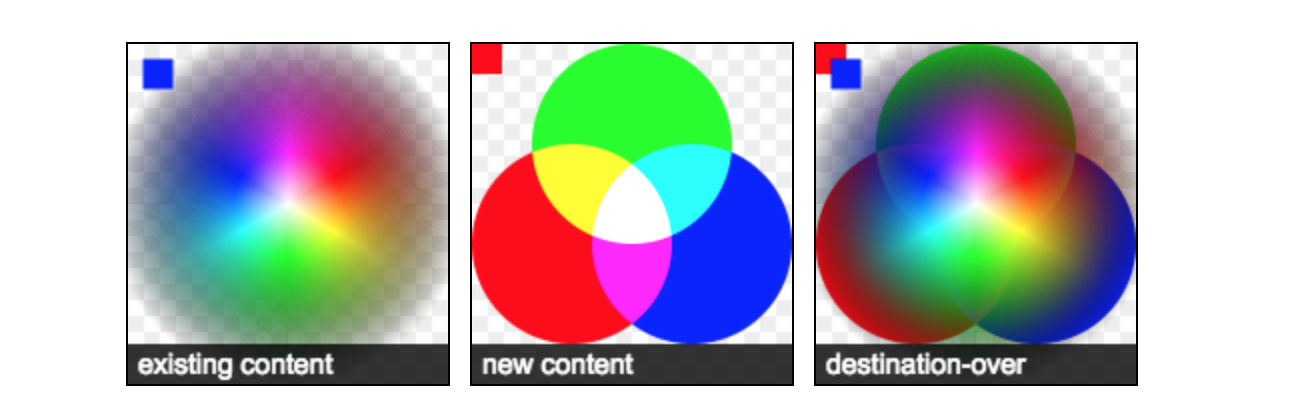
\includegraphics[scale=0.45]{Gambar/canvas_destination}
	\caption{Efek \textit{destination-over}}
	\label{fig:canvas_destination}
\end{figure}
			\end{itemize}
		\end{itemize}
		
		Beberapa \textit{method} yang dimiliki oleh kelas ini adalah sebagai berikut:
		\begin{itemize}
			\item \textbf{CanvasRenderingContext2D.clearRect(x, y, width, height)} \\
			Pada pengembangan Finger For Life, \textit{method} ini digunakan untuk menghilangkan gambar tertentu dari layar dengan tujuan untuk menampilkan gambar baru kelayar. Contoh implementasi dari \textit{method} ini adalah sebagai berikut:
\begin{lstlisting}[caption={Implementasi \textit{method clearRect()}}]
ctx.clearRect(0, 0, 900, 600);
\end{lstlisting}
\textit{Method} ini akan menghilangkan seluruh isi dari \textit{rectangle} pada \textit{canvas}, yang dimulai dari posisi (0,0), dengan lebar 600, dan panjang 900.			
			
			\item \textbf{CanvasRenderingContext2D.drawImage(image, dx, dy)} \\
			Pada pengembangan Finger For Life, \textit{method} ini digunakan untuk menggambar suatu grafis yang dibutuhkan didalam pengembangan aplikasi. Contoh implementasi dari \textit{method} ini adalah sebagai berikut:
\begin{lstlisting}[caption={Implementasi \textit{method drawImage()}}]
ctx.drawImage(image, 100, 100);
\end{lstlisting}
\textit{Method} ini akan menggambar variabel \textit{image} pada posisi (100,100).

			\item \textbf{CanvasRenderingContext2D.save()} \\
			Pada pengembangan Finger For Life, \textit{method} ini digunakan untuk menyimpan \textit{state} dari \textit{canvas} saat ini, sebelum \textit{state} tersebut dihilangkan untuk menaruh gambar yang baru. Tujuan dari proses ini adalah untuk membuat animasi pada permainan. Contoh implementasi dari \textit{method} ini adalah sebagai berikut:
\begin{lstlisting} [caption={Implementasi \textit{method save()}}]
ctx.save();
\end{lstlisting}	

			\item \textbf{CanvasRenderingContext2D.restore()} \\
			Pada pengembangan Finger For Life, \textit{method} ini digunakan untuk mengembalikan \textit{state} dari \textit{canvas} saat ini menjadi \textit{state} sebelumnya. \textit{Method} ini digunakan didalam proses animasi permainan. Contoh implementasi dari \textit{method} ini adalah sebagai berikut:
\begin{lstlisting}[caption={Implementasi \textit{method save()}}]
ctx.restore();
\end{lstlisting}
		\end{itemize}
	\end{enumerate}
	
	\item \textbf{jQuery} 
	\begin{enumerate}
		\item \textbf{submit(handler)} \\
		Pada pengembangan Finger For Life, \textit{method} ini digunakan untuk mengirimkan data kode \textit{room} yang sudah diisi oleh pengguna kedalam kolom. \textit{Method} ini akan digunakan pada tahap permintaan bergabung bagi pengguna. Contoh implementasi dari \textit{method} ini adalah sebagai berikut:
\begin{lstlisting}[caption={Implementasi \textit{method .submit()}}]
$('form').submit(function(e){
	e.preventDefault();
	socket.emit('requestToJoin', {
		id: socket.id,
		room: $('#code').val()
	});
});
\end{lstlisting}
\textit{Method} ini akan mengambil elemen \textit{form} dari berkas HTML, untuk mengambil data yang telah diisi oleh pengguna yang kemudian dikirimkan ke \textit{server}. Pada saat pengguna \textit{smartphone} menekan tombol \textit{send} pada layar, maka \textit{method} ini akan dieksekusi.
		
		\item \textbf{val()} \\
		Pada pengembangan Finger For Life, \textit{method} ini digunakan untuk mengambil nilai dari data yang telah diisi oleh pengguna kedalam kolom. \textit{Method} ini akan digunakan pada tahap permintaan bergabung bagi pengguna. Contoh implementasi dari \textit{method} ini adalah sebagai berikut:
\begin{lstlisting}[caption={Implementasi \textit{method val()}}]
var code = $('#code').val()
\end{lstlisting}
		\textit{Method} ini akan mengakses elemen HTML dengan \textit{id code}, kemudia mengambil data yang ada didalamnya untuk disimpan ke variabel \textit{code}.
		
		\item \textbf{html()} \\
		Pada pengembangan Finger For Life, \textit{method} ini digunakan untuk mengambil seluruh isi dari elemen HTML. \textit{Method} ini digunakan pada proses menampilkan seluruh halaman yang tersedia pada aplikasi web yang akan dibangun. Contoh implementasi dari \textit{method} ini adalah sebagai berikut:		
\begin{lstlisting}[caption={Implementasi \textit{method .html()}}]
var charMobileHtml = $("#charMobile").html();
\end{lstlisting}
		\textit{Method} ini akan mengakses elemen HTML yang memiliki \textit{id charMobile}, yang kemudian akan mengambil seluruh isi dari elemen tersebut untuk disimpan ke variabel \textit{charMobileHtml}.
		
		\item \textbf{preventDefault()} \\
		Pada pengembangan Finger For Life, \textit{method} ini digunakan untuk mencegah aksi \textit{default} yang akan dilakukan \textit{method submit()}, pada saat mengirim \textit{form} ke \textit{server}. \textit{Method} ini dieksekusi pada saat pengguna mengirimkan data kode \textit{room} untuk melakukan proses permintaan bergabung. Contoh implementasi dari \textit{method} ini adalah sebagai berikut:
\begin{lstlisting}[caption={Implementasi \textit{method preventDefault()}}]
$('form').submit(function(e){
	e.preventDefault();
});
\end{lstlisting}
		\textit{Method} ini akan mengakses elemen \textit{form} dari HTML, dan mencegah aksi \textit{default} dari \textit{method submit()} dilakukan. Aksi \textit{default} yang dilakukan adalah melakukan \textit{reload} pada halaman web.
	\end{enumerate}
	
	\item \textbf{The Content Template element} \\
	Pada pengembangan Finger For Life, <template> digunakan untuk menyimpan seluruh halaman-halaman yang diperlukan untuk pengembangan aplikasi permainan berbasis web ini. Pada proses implementasi, terdapat banyak <template> yang menyimpan halaman web yang berbeda-beda. Contoh implementasi dari elemen ini adalah sebagai berikut:
\begin{lstlisting}[caption={Implementasi elemen <template>}]
<template id="homePage">
<div class="titleContainer">
<div class="leftFing">
<img src="images/finga.png" id="leftFingImg">
</div>
	
<div class="wordContainer">
<div class="word">
<p>FINGER <br> FOR <br> LIFE</p>
</div>
	
<button id="startButton" onclick="startClicked()">START</button>
<button id="joinButton" onclick="joinClicked()">JOIN</button>
	
</div>
	
<div class="rightFing">
<img src="images/finga.png" id="rightFingImg">
</div>
</div>
</template>
\end{lstlisting}
Elemen ini memiliki \textit{id} dengan nama \textit{homePage}, dimana elemen ini dapat diakses dengan menggunakan jQuery, apabila perlu ditampilkan kelayar pengguna.

\end{enumerate}

\section{Analisis \textit{Use Case}}
\label{sec:usecase}

\subsection{Diagram \textit{Use Case}}
\label{subsec:diagram_usecase}

Diagram \textit{use case} pada permainan berbasis web yang akan dibangun hanya mengandung satu aktor, yaitu pemain. Diagram \textit{use case} dapat dilihat pada Gambar \ref{fig:usecase_pemain}.

\begin{figure}[H]
	\centering
	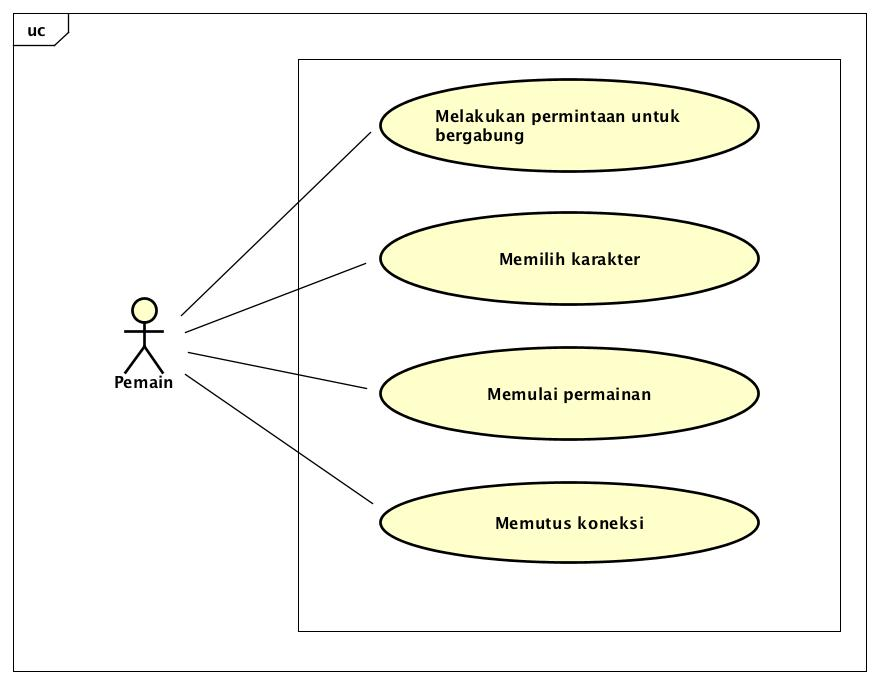
\includegraphics[scale=0.4]{Gambar/usecase_pemain}
	\caption{Diagram \textit{use case} pemain}
	\label{fig:usecase_pemain}
\end{figure}

Berdasarkan hasil analisis pada subbab \ref{sec:alur}, akan dibentuk empat \textit{use case} seperti berikut:

\begin{itemize}
	\item \textbf{Melakukan permintaan untuk bergabung}, pemain dapat bergabung dalam permainan dengan mengirimkan kode yang sudah disediakan \textit{browser PC} dengan menggunakan \textit{browser smartphone}.
	
	\item \textbf{Memilih karakter}, pemain dapat memilih karakter yang tersedia di \textit{browser smartphone}.
	
	\item \textbf{Memainkan permainan}, pemain dapat memainkan permainan dengan menekan tombol-tombol yang ada di \textit{smartphone}.
	
	\item \textbf{Mengakhiri permainan}, pemain dapat mengakhiri permainan dengan memutus koneksi Socket.io.
\end{itemize}

\subsection{Skenario \textit{Use Case}}

\begin{enumerate}
	\item \textbf{Melakukan Permintaan Untuk Bergabung}
	
	\begin{itemize}
		\item Nama: Melakukan permintaan untuk bergabung
		
		\item Aktor: Pemain
		
		\item Deskripsi: Melakukan permintaan untuk bergabung dengan \textit{room} yang sudah tersedia
		
		\item Kondisi awal: Pemain telah membuka halaman permintaan bergabung pada \textit{browser smartphone} dan mengisi \textit{form} dengan kode yang telah disediakan
		
		\item Kondisi akhir: Pemain bergabung kedalam \textit{room}
		
		\item Skenario utama: 
		

\begin{tabular}{ |p{1cm}|p{4cm}|p{4cm}|}
	\hline
	No & Aksi Aktor & Reaksi Sistem \\ \hline
	1 & Pemain mengisi \textit{form} dengan kode \textit{room} dan menekan tombol \textit{send} & Sistem mendapatkan kode \textit{room} dan memproses kode tersebut, kemudian memberikan \textit{feedback} kepada pemain. \\ \hline
\end{tabular}

		\item Eksepsi: Pemain bergabung kedalam \textit{room}.

		
	\end{itemize}
	
	\item \textbf{Memilih Karakter}
	
	\begin{itemize}
		\item Nama: Memilih karakter
		
		\item Aktor: Pemain
		
		\item Deskripsi: Memilih karakter yang ditampilkan pada \textit{browser smartphone}
		
		\item Kondisi awal: Pemain telah bergabung kedalam \textit{room}
		
		\item Kondisi akhir: Pemain menetapkan karakter yang akan dimainkan
		
		\item Skenario utama:
		
\begin{tabular}{ |p{1cm}|p{4cm}|p{4cm}|}
	\hline
	No & Aksi Aktor & Reaksi Sistem \\ \hline
	1 & Pemain memilih karakter yang tersedia dan menetapkan karakter tersebut. & Sistem menerima karakter yang dipilih dan menetapkan karakter yang dipilih oleh pemain \\ \hline
\end{tabular}

	\item Eksepsi: Karakter muncul dilayar \textit{PC}.
		
	\end{itemize}
	
	\item \textbf{Memainkan Permainan}
		
		\begin{itemize}
			\item Nama: Memainkan permainan
			
			\item Aktor: Pemain
			
			\item Deskripsi: Memainkan permainan dengan menekan tombol-tombol pada \textit{browser smartphone} untuk menggerakan karakter
			
			\item Kondisi awal: Pemain telah menetapkan karakter permainan
			
			\item Kondisi akhir: Pemain memainkan permainan dengan menggerakan karakter
			
			\item Skenario utama:

\begin{tabular}{ |p{1cm}|p{4cm}|p{4cm}|}
	\hline
	No & Aksi Aktor & Reaksi Sistem \\ \hline
	1 & Pemain menekan tombol telapak kaki berulang-ulang & Sistem menangkap \textit{event} menekan tombol telapak kaki dan menggerakan karakter milik pemain \\ \hline
\end{tabular}
			
			\item Karakter bergerak dari garis awal hingga akhir.	
			
		\end{itemize}
	
	\item \textbf{Memutus Koneksi}
	
		\begin{itemize}
			\item Nama: Memutus koneksi
			
			\item Aktor: Pemain
			
			\item Deskripsi: Memutus koneksi dengan keluar dari \textit{browser} atau menekan tombol \textit{exit} saat telah selesai bermain
			
			\item Kondisi awal: Pemain telah selesai bermain
			
			\item Kondisi akhir: Pemain keluar dari permainan dan koneksi terputus
			
			\item Skenario utama:
			
\begin{tabular}{ |p{1cm}|p{4cm}|p{4cm}|}
	\hline
	No & Aksi Aktor & Reaksi Sistem \\ \hline
	1 & Pemain menekan tombol \textit{exit} pada halaman terakhir atau menutup \textit{browser} & Sistem akan menangkap \textit{event} tombol \textit{exit} ditekan dan memutus koneksi pemain \\ \hline
\end{tabular}
			
			\item Eksepsi: Seluruh \textit{client} keluar dari permainan.
		\end{itemize}
\end{enumerate}


\section{Analisis Arsitektur Finger For Life}
Arsitektur Finger For Life dapat dilihat pada Gambar \ref{fig:ars_fingerforlife} . Jumlah \textit{Client} dalam permainan ini adalah tiga. \textit{Client} tersebut antara lain \textit{host}, \textit{player 1}, dan \textit{player 2}. Apabila \textit{player 1} akan mengirimkan data untuk diproses oleh \textit{host}, maka data tersebut akan dikirimkan terlebih dahulu kepada \textit{server}, kemudian dilanjutkan kepada \textit{host}.

\begin{figure}[H]
	\centering
	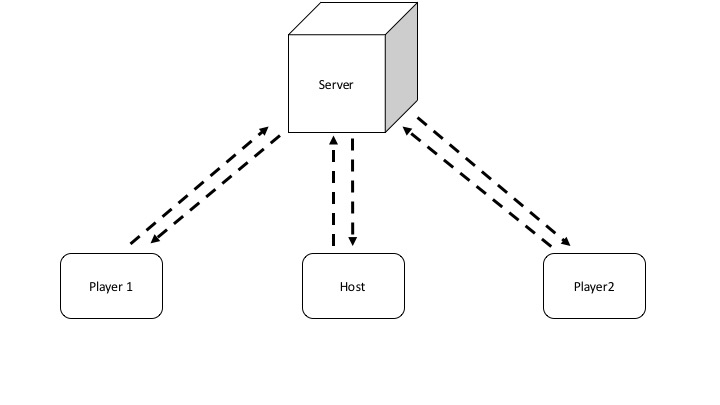
\includegraphics[scale=0.45]{Gambar/ars_fingerforlife}
	\caption{Arsitektur Finger For Life}
	\label{fig:ars_fingerforlife}
\end{figure}

Komunikasi antara \textit{client} dengan \textit{client} tidak dapat dilakukan secara langsung. Komunikasi tersebut harus melewati \textit{server} terlebih dahulu. 

Finger For Life dibangun diatas Node.js. Seluruh berkas serta direktori yang dibutuhkan untuk membangun aplikasi permainan ini diatur dengan menggunakan Express.js. Proses pengiriman dan penerimaan data secara \textit{realtime} dilakukan menggunakan Socket.io. Dalam permainan ini, animasi akan dilakukan dengan menggunakan Canvas API. Seluruh proses memodifikasi elemen HTML akan dilakukan dengan menggunakan jQuery. Halaman-halaman yang dibutuhkan untuk ditampilkan kelayar akan diatur dengan menggunakan The Content Template element.

\section{Analisis Socket.io}
Pada pengembangan Finger For Life digunakan banyak fitur yang telah disediakan oleh Socket.io. Teknologi ini digunakan untuk proses sinkronisasi antara \textit{smartphone} dengan \textit{PC} dan komunikasi secara \textit{real-time} antara \textit{client} dan \textit{server}. Seperti yang sudah dijelaskan pada subbab \ref{sec:alur}, ada beberapa tahap yang harus dilakukan sebelum dapat memainkan aplikasi permainan berbasis web ini. Tahap tersebut banyak menggunakan pustaka Socket.io dalam proses implementasinya.

Subbab-subbab ini akan menjelaskan bagaimana teknologi Socket.io digunakan dalam implementasi Finger For Life pada tahap-tahap yang harus dilakukan.
\begin{enumerate}
	\item \textbf{Komunikasi antara \textit{client} dan \textit{server}} \\
	Pada aplikasi permainan berbasis web ini, akan banyak dibutuhkan proses komunikasi antara sesama \textit{client} maupun dengan \textit{server}. Komunikasi yang dilakukan harus secara \textit{real-time}, agar interaksi didalam permainan dapat berjalan pada saat permainan dimainkan.
	
	Interaksi tersebut akan dilakukan berdasarkan \textit{event}. Suatu \textit{event} akan dipancarkan kedalam suatu \textit{stream}, dimana \textit{stream} akan berisi berbagai \textit{event} yang telah dipancarkan, yang menunggu untuk ditangkap oleh fungsi tertentu. Pada saat \textit{client} akan berkomunikasi dengan \textit{client} lain, maka \textit{event} yang dipancarkan akan ditangkap oleh \textit{server} sebelum kemudian dilanjutkan kepada \textit{client} lain. Arsitektur interaksi antara \textit{client} dan \textit{server} dapat dilihat pada Gambar \ref{fig:ars_socketio}.
\begin{figure}[H]
	\centering
	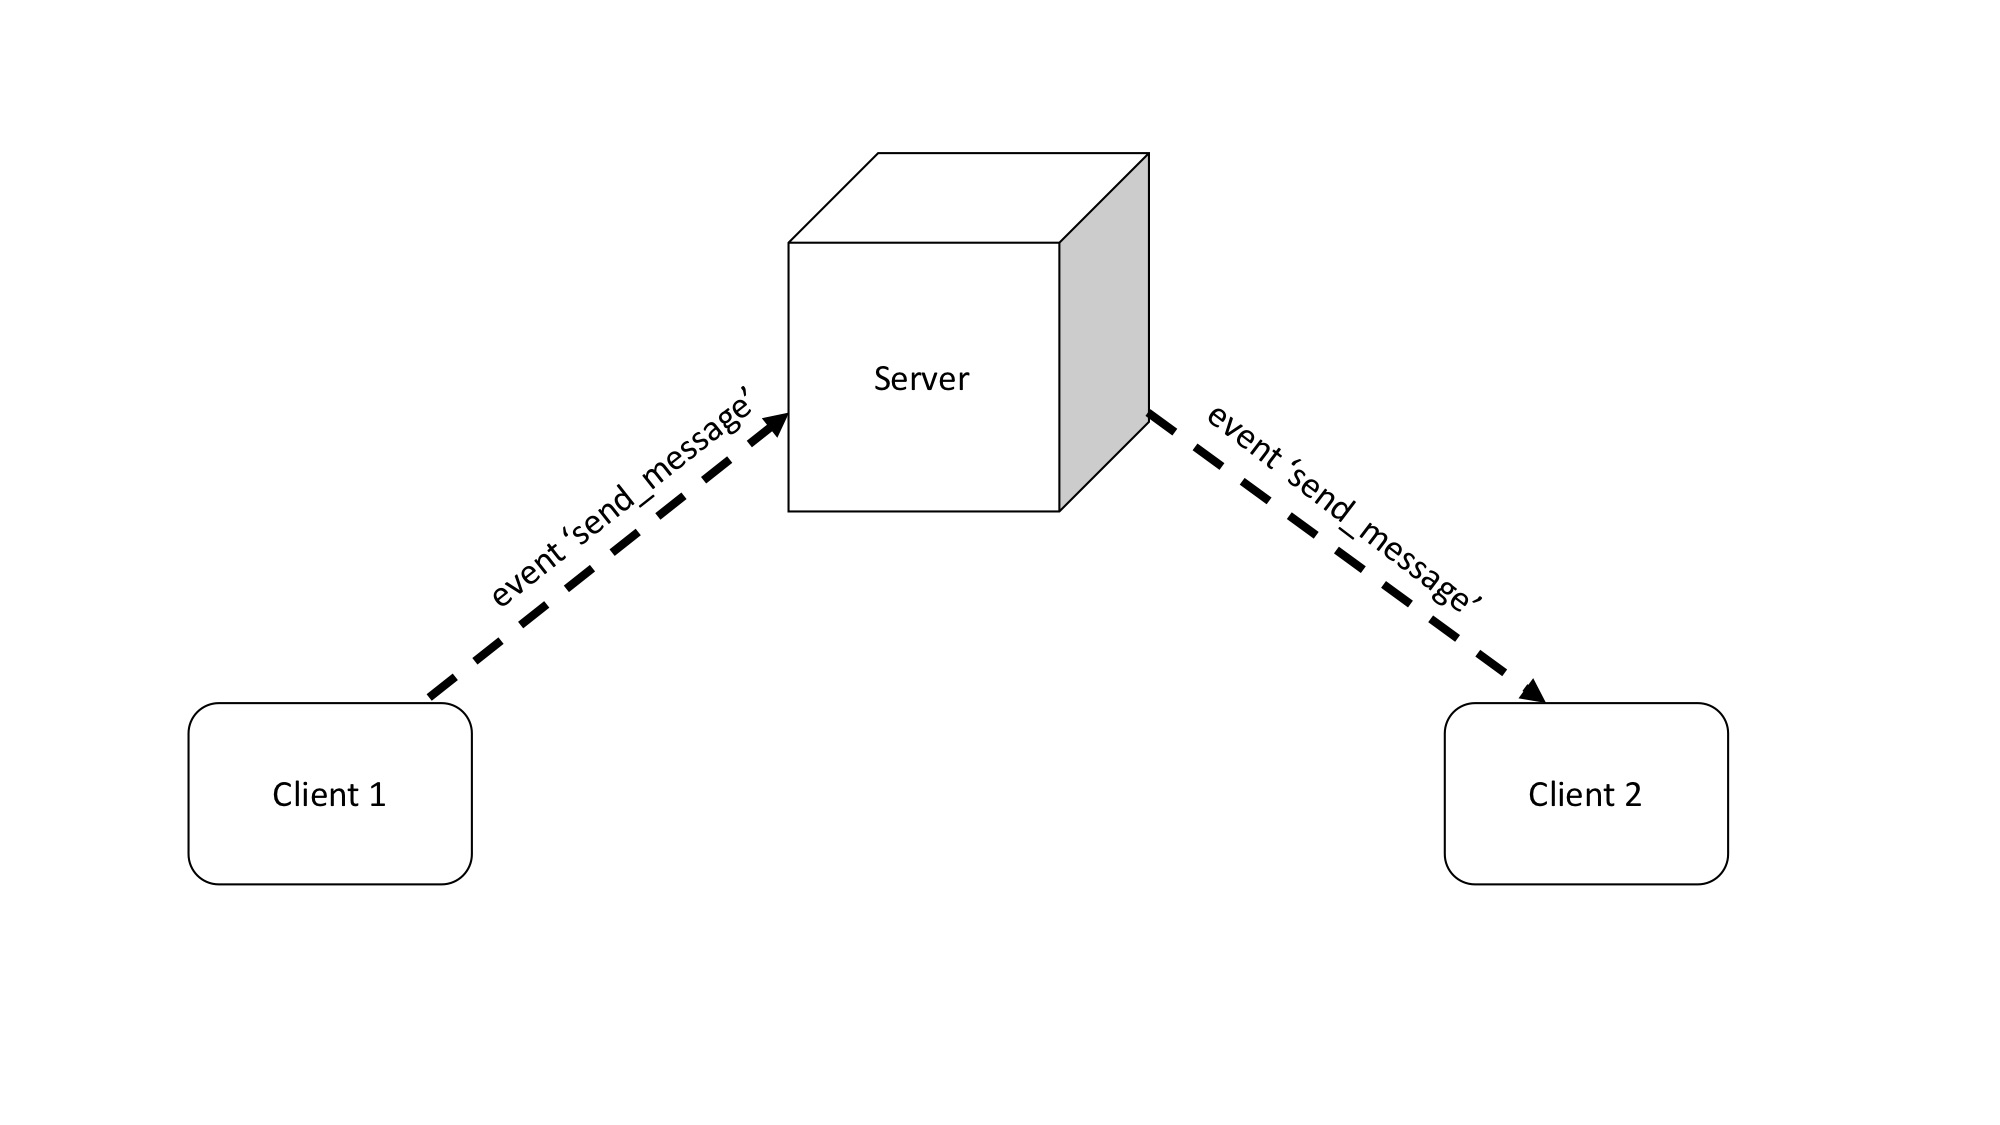
\includegraphics[scale=0.2]{Gambar/ars_socketio}
	\caption{Arsitektur interaksi \textit{client} dan \textit{server}}
	\label{fig:ars_socketio}
\end{figure}	
	Agar proses tersebut dapat dilakukan, maka fitur yang dimiliki oleh Socket.io akan digunakan. Fitur-fitur tersebut adalah sebagai berikut:
	
	\begin{itemize}
		\item \textbf{socket.emit(eventName[, ...args][, ack])} \\ 
		\textit{Method} ini akan memancarkan \textit{event} dengan nama \textit{eventName}, dimana \textit{event} tersebut dapat ditangkap oleh \textit{client} maupun \textit{server} dengan menggunakan fungsi tertentu. Apabila \textit{event} yang telah dipancarkan tidak ditangkap oleh siapapun, maka \textit{event} tersebut akan disimpan oleh \textit{stream} hingga suatu sesi selesai yang kemudian akan dihancurkan.
		
		\item \textbf{socket.on(eventName, callback)} \\
		\textit{Method} ini akan menangkap \textit{event} yang namanya sesuai dengan parameter \textit{eventName}. \textit{Method} ini yang akan menangkap suatu \textit{event} yang telah dipancarkan kedalam \textit{stream}. Setelah \textit{event} tersebut ditangkap, maka fungsi \textit{callback} akan dieksekusi.
	\end{itemize}
Contoh implementasi dari proses interaksi antara \textit{client} dan \textit{server} adalah sebagai berikut:
\begin{lstlisting}[caption={Potongan kode pada bagian \textit{client}}, label={lst:interaksi_client}, captionpos=b]
socket.emit('requestToJoin', {
	id: socket.id,
	room: $('#code').val()
});

socket.on('joinSucceed', function(msg){
	var messages = document.getElementById("joined");
	messages.innerHTML = msg;
});

socket.on('joinRejected', function(msg){
	var messages = document.getElementById("joined");
	messages.innerHTML = msg;
});
\end{lstlisting}
Potongan kode ini menunjukan suatu \textit{client} yang memancarkan \textit{event requestToJoin} dengan data-data yang dikirimkan. \textit{Event} tersebut akan ditangkap oleh \textit{server} untuk dilakukan pengecekan terhadap data yang dikirimkan. Selain itu, \textit{client} memiliki \textit{event handler} yang akan menangkap \textit{event joinRejected} dan \textit{joinSucceed}.


\begin{lstlisting}[caption={Potongan kode pada bagian \textit{server}}, label={lst:interaksi_server}, captionpos=b]
socket.on('requestToJoin', function(msg){
var check = users.isRoomExist(msg.room);

if (check === 1) {
io.to(msg.room).emit('requestAccepted', 'Client has joined the room.');
}else{
socket.emit('joinRejected', 'The room is not exist');
}
});
\end{lstlisting}
Pada potongan kode ini, \textit{server} akan menangkap \textit{event requestToJoin} yang dipancarkan oleh \textit{client}. Apabila \textit{client} telah memancarkan \textit{event} tersebut, maka \textit{server} akan menangkap \textit{event} dan mengeksekusi fungsi \textit{callback}. \textit{Server} kemudian akan melakukan pengecekan terhadap data \textit{msg} yang diterima. Apabila pengecekan menghasilkan angka satu, maka \textit{server} akan memancarkan \textit{event requestAccepted} kepada \textit{client} lain yang berada didalam \textit{room}. Apabila pengecekan tidak menghasilkan angka satu, maka \textit{server} akan memancarkan \textit{event joinRejected} kepada satu \textit{socket} yang sedang melakukan koneksi kepada \textit{server}.

\begin{lstlisting}[caption={Proses \textit{event} diterima}, label={lst:req_accepted}, captionpos=b]
socket.on('requestAccepted', function(msg){
	showMessage(msg);
});
\end{lstlisting}
Potongan kode ini menunjukan suatu \textit{client} yang akan menangkap \textit{event requestAccepted} yang dikirimkan oleh \textit{server}. \textit{Client} kemudian akan mengeksekusi fungsi \textit{callback} untuk mengolah data yang dikirimkan.
	
	\item \textbf{Sinkronisasi \textit{PC} dan \textit{Smartphone}} \\
	Pada permainan Finger For Life terdapat tahap permintaan bergabung yang dilakukan oleh \textit{PC} dan \textit{smartphone}. Tahap tersebut merupakan proses sinkronisasi yang harus dilakukan agar \textit{smartphone} dan \textit{PC} dapat tersambung dan dapat berkomunikasi satu sama lain. Kedua gawai tersebut dapat tersambung dengan menggunakan Socket.io. Ada beberapa langkah yang harus dilakukan, langkah-langkah tersebut antara lain:
	\begin{itemize}
		\item \textbf{Koneksi Socket.io} \\
		Sebelum \textit{PC} dan \textit{smartphone} tersambung, kedua gawai tersebut harus terkoneksi dengan Socket.io. Proses melakukan koneksi terhadap Socket.io dilakukan pada saat halaman web mengakses halaman permintaan bergabung. Pada saat kedua gawai mengakses halaman tersebut, proses yang terjadi adalah sebagai berikut:
		\begin{itemize}
			\item Didalam berkas \textit{syncScript.js} \ref{sec:direktori} dan \textit{mobileScript.js} \ref{sec:direktori}, terdapat variabel yang memulai \textit{client} untuk melakukan koneksi kepada Socket.io. Variabel tersebut adalah sebagai berikut:
\begin{lstlisting}[caption={Potongan kode untuk mendapatkan fungsi Socket.io pada \textit{client}}]
var socket = io();
\end{lstlisting}
			Variabel \textit{socket} akan mendapatkan fungsi-fungsi milik Socket.io yang telah tersedia, yang dapat dipakai pada bagian \textit{client}. Apabila \textit{PC} dan \textit{smartphone} telah mengakses halaman permintaan bergabung, maka kedua gawai tersebut telah terkoneksi dengan Socket.io. Walaupun sudah terkoneksi, kedua gawai tersebut belum dapat berkomunikasi satu sama lain.
		\end{itemize}
	
		\item \textbf{Sinkronisasi \textit{PC} dan \textit{Smartphone}} \\
		\textit{PC} akan menyediakan kode yang harus dikirimkan oleh \textit{smartphone}. Kode tersebut merupakan kode \textit{room} yang dibutuhkan untuk proses sinkronisasi antara \textit{PC} dan \textit{smartphone}. Kode \textit{room} akan dibangkitkan secara acak pada halaman \textit{sync}. Kode tersebut dibangkitkan dengan cara seperti berikut:
\begin{lstlisting}[caption={Proses membangkitkan kode \textit{room}}, label={lst:bangkit_kode}, captionpos=b]
function getRandInt(){
text = Math.floor(Math.random() * (999999 - 111111)) + 111111;
document.getElementById("roomId").innerHTML = text;
}
\end{lstlisting}
		Kode yang akan dibangkitkan secara acak berjumlah enam dijit angka, dimana angka tersebut berada didalam rentang 000000 hingga 999999. Pada saat kode \textit{room} telah dibangkitkan, \textit{PC} secara otomatis akan langsung bergabung kedalam \textit{room} tersebut. Langkah tersebut dapat dilakukan seperti berikut:
\begin{lstlisting}[caption={Proses \textit{host} bergabung kedalam room}, label={host_gabung}, captionpos=b]
function getRandInt(){
	text = Math.floor(Math.random() * (999999 - 111111)) + 111111;
	document.getElementById("roomId").innerHTML = text;

	var roomString = text.toString();

	socket.emit('hostJoinRoom', {
		id: socket.id,
		room: roomString
	});
}
\end{lstlisting}
		\textit{PC} akan memancarkan \textit{event hostJoinRoom} yang akan ditangkap oleh \textit{server}. \textit{Event} tersebut mengirimkan data berupa identifikasi unik milik \textit{client}, dan kode \textit{room} yang telah dibangkitkan. \textit{Server} akan menangkap \textit{event} tersebut dan menambahkan \textit{host} kedalam \textit{room} yang telah dibangun. Proses tersebut dilakukan sebagai berikut:
\begin{lstlisting}[caption={\textit{Server} menerima \textit{event} dari \textit{host}}, label={lst:server_acc_host}, captionpos=b]
socket.on('hostJoinRoom', (msg) => {
	socket.join(msg.room);
	users.removeUser(msg.id);
	users.addUser(msg.id, msg.room);
});
\end{lstlisting}
		\textit{Event hostJoinRoom} akan ditangkap oleh \textit{server} kemudian akan mengeksekusi fungsi yang ada didalamnya. \textit{Server} akan menambahkan \textit{host} kedalam \textit{room} dengan menggunakan \textit{socket.join(msg.room)}. Kemudian \textit{host} akan ditambahkan kedalam \textit{array} yang berada didalam kelas Users. Array tersebut berisi daftar \textit{client} yang telah memiliki \textit{room}. Proses tersebut dilakukan dengan menggunakan \textit{users.addUser(msg.id, msg.room)}. Dengan melakukan proses ini, maka \textit{room} telah dibangkitkan, dan \textit{host} telah tergabung didalamnya.
		
		Setelah kode \textit{room} dibangkitkan, maka akan ditampilkan kelayar \textit{PC}. Pengguna akan memasukan kode tersebut ke kolom yang berada dihalaman \textit{smartphone} untuk dikirimkan ke \textit{server}. Proses ini merupakan proses sinkronisasi yang dibutuhkan antara \textit{PC} dan \textit{smartphone}. Proses pengiriman kode \textit{room} akan dilakukan dengan cara berikut:
\begin{lstlisting}[caption={Proses permintaan bergabung pada \textit{client}}, label={lst:client_req}, captionpos=b]
function requestToJoin(){
	$('form').submit(function(e){
		e.preventDefault();
		socket.emit('requestToJoin', {
			id: socket.id,
			room: $('#code').val()
		});
	});
}
\end{lstlisting}
		\textit{Smartphone} akan mengirimkan kode \textit{room} dengan memancarkan \textit{event requestToJoin}. Kode \textit{room} yang telah diisi didalam kolom akan diambil dengan menggunakan jQuery. Proses tersebut dilakukan dengan menggunakan \textit{jQuery('\#code').val()}. \textit{Event requestToJoin} akan mengirim data identifikasi unik Socket.io milik \textit{client} dan kode \textit{room}. \textit{Event} tersebut akan ditangkap oleh \textit{server} yang kemudian akan dilakukan proses verifikasi. Proses tersebut akan dilakukan seperti berikut:
\begin{lstlisting}[caption={Proses verifikasi}, label={lst:prosesVerifikasi},captionpos=b]
socket.on('requestToJoin', function(msg){
	var check = users.isRoomExist(msg.room);

	if (check === 1) {
		socket.join(msg.room);
		users.removeUser(msg.id);
		users.addUser(msg.id, msg.room);

		io.to(user.room).emit('requestAccepted', msg);
		socket.emit('joinSucceed', 'Welcome to the game :)');

	}else{
		socket.emit('joinRejected', 'The room is not exist');
	}
})
\end{lstlisting}
		\textit{Event} ini akan memeriksa apakah kode yang dikirimkan oleh \textit{smartphone} sesuai dengan data \textit{room} yang ada didalam \textit{array}. Pengecekan tersebut dilakukan dengan menggunakan \textit{var check = users.isRoomExist(msg.room)}. Apabila \textit{room} sesuai, maka \textit{smartphone} dapat bergabung kedalam \textit{room}, apabila tidak sesuai, maka \textit{smartphone} tidak dapat bergabung. Dengan bergabungnya \textit{smartphone} kedalam \textit{room}, maka proses sinkronisasi antara \textit{smartphone} dan \textit{PC} telah terpenuhi. Dengan begitu, kedua gawai tersebut dapat melakukan komunikasi satu sama lain.
		
	\end{itemize}
\end{enumerate}
